\chapter{Fenómenos de transporte en semiconductores}



En este tema estudiarmemos los fenómenos de transporte en semiconductores, que son varios. Dedicaremos una sección a cada uno de ellos:

\begin{itemize}
	\item Arrastre.
	\item Difusión.
	\item Generación.
	\item Recombinación.
	\item Emisión termoiónica.
	\item Trasmisión túnel.
	\item Ionización por impacto.
\end{itemize}
Además veremos \textit{ecuaciones básicas de trasnporte} y métodos de medida de parámetros como resistividad, movilidades, concentración, tiempos de vida, etc.


%%%%%%%%%%%%%%%%%%%%%%%%%%%%%%%%%%%%%%%%%%%%%%%%%%%%%%%%%%%%%%%%%%%%%%%
%%%%%%%%%%%%%%%%%%%%%%%%%%%%%%%%%%%%%%%%%%%%%%%%%%%%%%%%%%%%%%%%%%%%%%%
%%%%%%%%%%%%%%%%%%%%%%%%%%%%%%%%%%%%%%%%%%%%%%%%%%%%%%%%%%%%%%%%%%%%%%%
%%%%%%%%%%%%%%%%%%%%%%%%  TEMA 1 %%%%%%%%%%%%%%%%%%%%%%%%%%%%%%%%%%
%%%%%%%%%%%%%%%%%%%%%%%%%%%%%%%%%%%%%%%%%%%%%%%%%%%%%%%%%%%%%%%%%%%%%%%
%%%%%%%%%%%%%%%%%%%%%%%%%%%%%%%%%%%%%%%%%%%%%%%%%%%%%%%%%%%%%%%%%%%%%%%
%%%%%%%%%%%%%%%%%%%%%%%%%%%%%%%%%%%%%%%%%%%%%%%%%%%%%%%%%%%%%%%%%%%%%%%

\section{Arrastre}

\subsection{Introducción: modelo de arrastre y difusión}

El \textbf{modelo de arrastre-difusión} considera que las corrientes en el interior del semiconductor se debe exclusivamente a dos componentes: arrastre y difusión.

\begin{itemize}
	\item \textbf{Arrastre:} movimiento de los portadores provocado por campos eléctricos externos e internos.
	\item \textbf{Difusión:} movimiento de portadores debido a gradientes de concentración debido a gradientes de concentracion. En la difusión los portadores se desplazarán de donde son mayoritarios a donde son minoritarios.
\end{itemize}
Así pues, según este modelo, las corrientes de portadores electrón $J_n$ y de portadores hueco $J_p$ serán iguales a la suma de las componentes de arrastre y difusión:

\begin{equation}
	J_n =  {J_n}|_{\text{arrastre}} + {J_n}|_{\text{difusión}} \tquad
	J_p =  {J_p}|_{\text{arrastre}} + {J_p}|_{\text{difusión}}
\end{equation}
siendo la \textit{corriente total} la suma de ambas componentes:

\begin{equation}
	J = J_n + J_p
\end{equation}

\subsection{Corriente de arrastre}

Si no aplicamos ninguna fuerza externa, el movimiento de los electrones a tempeartura no nula será un proceso aleatorio, en el que se sucederán colisiones con átomos de la red, impurezas, fonones, fotones... de tal manera que \textit{el movimiento efectivo es nulo}. Sin embargo los electrones si poseen velocidad, la cual podemos calcular, en virtud del \textit{teorema de equipartición}, tal que por cada grado de libertad del electrón le asignamos $kT/2$ de energía cinética. Como en el modelo de semiconductores, los huecos y electrones en las bandas de valencia y conducción son partículas libres (con masa efectiva diferente a $m_e$, pero partículas libres a fin de cuentas), podemos aplicarles el teorema de equipartición, tal que:

\begin{equation}
	\frac{1}{2} m^* v_{th}^2 = \frac{3}{2} kT
\end{equation}
siendo $v_{th}$ la \textit{velocidad media de cada partícula}. Cuando aplicamos un campo eléctrico $\Ecal$, todos los portadores experimentarán una fuerza $q\Ecal$, que lo acelera entre las sucesivas colisiones. Esta fuerza aplicada sobre el semiconductor provocará un desplazamiento neto de electrones en la dirección opuesta al campo y de huecos en la dirección del campo. Definimos entonces dos parámetros fundamentales: \textbf{camino medio recorrido} $\lambda$, que es la distancia media entre dos colisiones $(\sim 10^{-5} \cm$) y el \textbf{tiempo medio recorrido} $\tau$, que es el tiempo medio entre dos colisiones ($\sim 10^{-12} s$).

Supongamos entonces que los portadores se mueven a una velocidad constante $v_a$ (que lógicamente dependerá de la temperatura, de la fuerza del campo...). Como hemos visto en el tema anterior, un hueco es una partícula virtual igual al electrón en todo exceptuando que tiene carga positiva. Si consideramos que el electrón se mueve a una velocidad constante $v_a$, el hueco también lo hará. En ese caso la densidad de corriente no es más que:

\begin{equation}
	J_n|_{\text{arrastre}} = -qnv_a \tquad 	J_p|_{\text{arrastre}} = qpv_a
\end{equation}
siendo $q$ la carga. Tal y como hemos dicho, la velocidad $v_a$ no es una constante del material, sino que depende de variables tales como la temperatura, el grado de impurezas o de la intensidad del campo. De manera experimental se sabe, que bajo campos no muy intensos, la velocidad tiene una dependencia lineal con el campo eléctrico, véase \cref{Fig:02-01}.

\begin{figure}[h!] \centering
	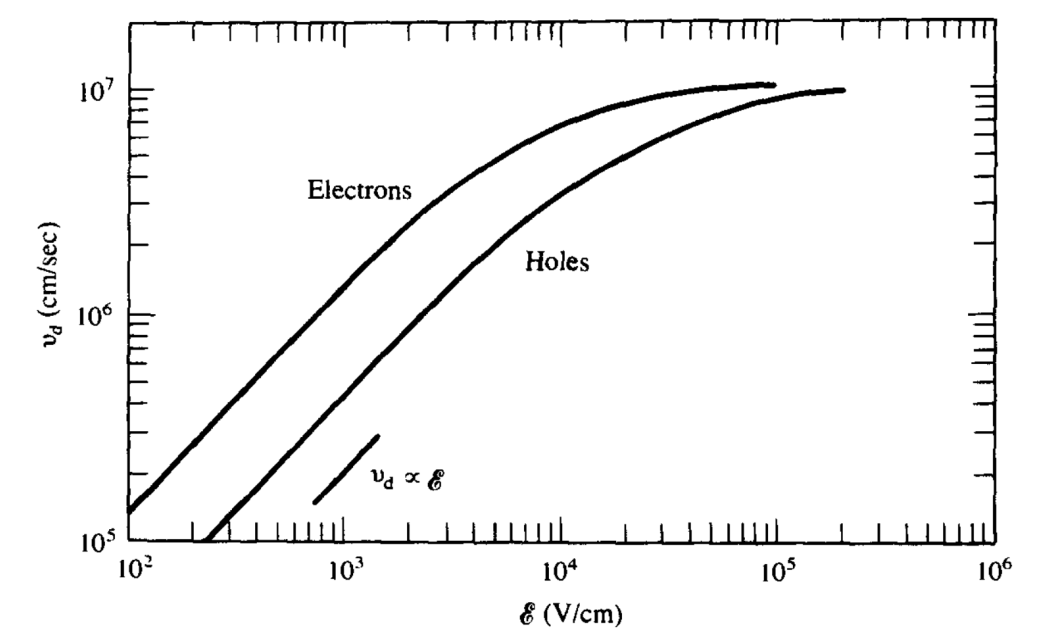
\includegraphics[width=0.9\linewidth]{Cuerpo/Ch_02/02_Movilidad_E.png}
	\caption{Movilidad frente a campo eléctrico. Véase que en la región de campo débil sigue una ecuación lineal, hasta que en campo fuerte se hace constante.}
	\label{Fig:02-01}
\end{figure}
La constante que relaciona la velocidad y el campo eléctrico se llama \textbf{movilidad} y se denota por $\mu$. Así pues, $\mu_n$ es la movilidad del electrón y $\mu_p$ la del hueco, y verifican:

\begin{equation}
	v_n = - \mu_n \Ecal \tquad v_p = \mu_p \Ecal
\end{equation}
midiéndose en $\cm^2/$Vs. Entonces la corriente de arrastre es:

\begin{equation}
	J_{\text{arrastre}} = qn\mu_n \Ecal + qp\mu_p \Ecal = q(n\mu_n+p\mu_p)\Ecal
\end{equation}
\subsection{Dispersión: efectos en la movilidad}

La movilidad, a su vez, depende del grado de dispersión. Si la dispersión es muy baja la movilidad es muy alta: los electrones chocan poco y se pueden acelerar mucho. Como fuentes de dispersión tenemos: \textit{fonones, átomos dopantes ionizados, aleaciones, imperfecciones en la red, defectos en las interfaces...} Los fenómenos que más influencia tienen son:

\begin{itemize}
	\item Dispersión por choques entre portadores (poca influcencia).
	\item Dipsersión por la red cristalina (choques de los portadores con los átomos de la red, que dominan a alta temperatura).
	\item Dispersión por dopantes ionizadas (choques con impurezas donadores o aceptadoras, que dominan a baja temperatura).
\end{itemize}
Consecuentemente tenemos dos efectos principales, el efecto debido a las impurezas y el efecto debido a los fonones. La probabildiad de colisión por unidad de tiempo global es la suma de las probabilidades parciales de cada tipo de colisión, según la \textit{regla matthiessen}:

\begin{equation}
	\frac{1}{\tau_c} = \frac{1}{\tau_c|_{\text{fonones}}}+\frac{1}{\tau_c|_{\text{impurezas}}}
\end{equation}
Los fonones aumentan como $T^{3/2}$
Y en términos de la movilidad:

\begin{equation}
	\frac{1}{\mu}=\frac{1}{\mu_F}+\frac{1}{\mu_I}
\end{equation}
lógicamente esto es \textit{generalizable}, pudiendo incluir los mecanismos de dispersión. Como podemos ver en la imagen \cref{Fig:02-02}, a altas temperautras la movilidad se reduce como $T^{-3/2}$ y a bajas temperaturas aumenta como $T^{3/2}$.

\begin{figure}[h!] \centering
	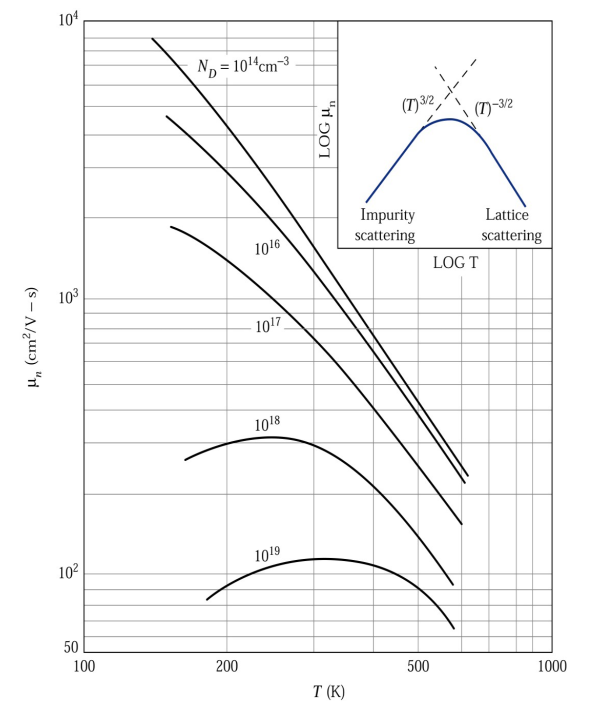
\includegraphics[width=0.6\linewidth]{Cuerpo/Ch_02/02_Movilidad.png}
	\caption{Movilidad en función de $T$.}
	\label{Fig:02-02}
\end{figure}

\subsubsection{Dispersión por impurezas}

Las impurezas ionizadas ocurren cuando el portador pasa cerca de un dopante ionizado debido a la fuerza de Coulomb. La probabilidad del choque con los dopantes ionizadas depende de la concentación total (suma de aceptores y donadores), dominando a baja temperatura $N_I \equiv N_A^- + N_D^+$. A diferencia de la dispersión por fonones, esta se \textit{reduce al aumentar la temperatura}, ya que los portadores van más rápido y pasab menos tiempo cerca de los dopantes. Teóricamente la movilidad debida a dopantes ionizadas crece con $T^{3/2}/N_I$. En resumen: domina a altos dopados (Si) y a bajas temperaturas. El valor de la movilidad en estes casos está dado por la siguiente ecuación: 

\begin{equation}
	\mu = \mu_{\min} + \frac{\mu_0}{1+\parentesis{\frac{N}{N_{\text{ref}}}}^{\alpha}}  
\end{equation}
siendo constantes la mayor parte de los términos (constantes que dependen de la temperatura y la masa efectiva). La única variable sería $N$, la concentración de impurezas ($N_D$ o $N_A$). Los demas parámetros dependen de $\theta=N_A/N_D$ y de $T$.

\subsubsection{Dispersión por fonones}

La dispersión por fonones viene a ser la dispersión por vibracioens en la red cristalina. Ocurren a temperaturas mayores al cero absoluto, aumentrando progresivamente con un ratio de $T^{3/2}$. Estas vibraciones modifican el potencial periódico, y permite intercambiar energía entre portadores y los núcleos del cristal. Dado que aumenta con $T^{3/2}$, tenemos que $\mu_{\text{fon}} \propto T^{-3/2}$.


\subsection{Resistividad y movilidad}

La \textbf{resistividad} ($\rho$) se define como la constante de proporcionalidad entr el campo eléctrico aplicado y la corriente total de carga por unidad de área que fluye en el mismo (suponiendo un material homogéneo). Al inverso de la resistividad lo llamamos \textbf{conductividad} ($\sigma$) tal que

\begin{equation}
	\sigma \equiv \frac{1}{\rho}
\end{equation}
Como sabemos $\Jn_{\text{arrastre}}=q(\mu_nn+\mu_pp)\Encal$. Entonces podemos relacionar la resistividad/conductividad de un material con la movilidad, tal que

\begin{equation}
	\rho = \frac{1}{q(\mu_n n + \mu_p p)}
\end{equation}

\subsection{Curvatura de bandas}

El campo eléctrico se puede estudiar y entender como el gradiente de una función llamada \textit{potencial escalar} que representa la energía por unidad de carga. Así pues, la acción de un campo eléctrico en un semiconductor hace que aparezca una diferencia de energía entre los diferentes puntos del semiconductor, haciendo que las bandas a lo largo del semiconductor no tengan la misma energía, tal y como podemos ver en .

\begin{figure}[h!] \centering
	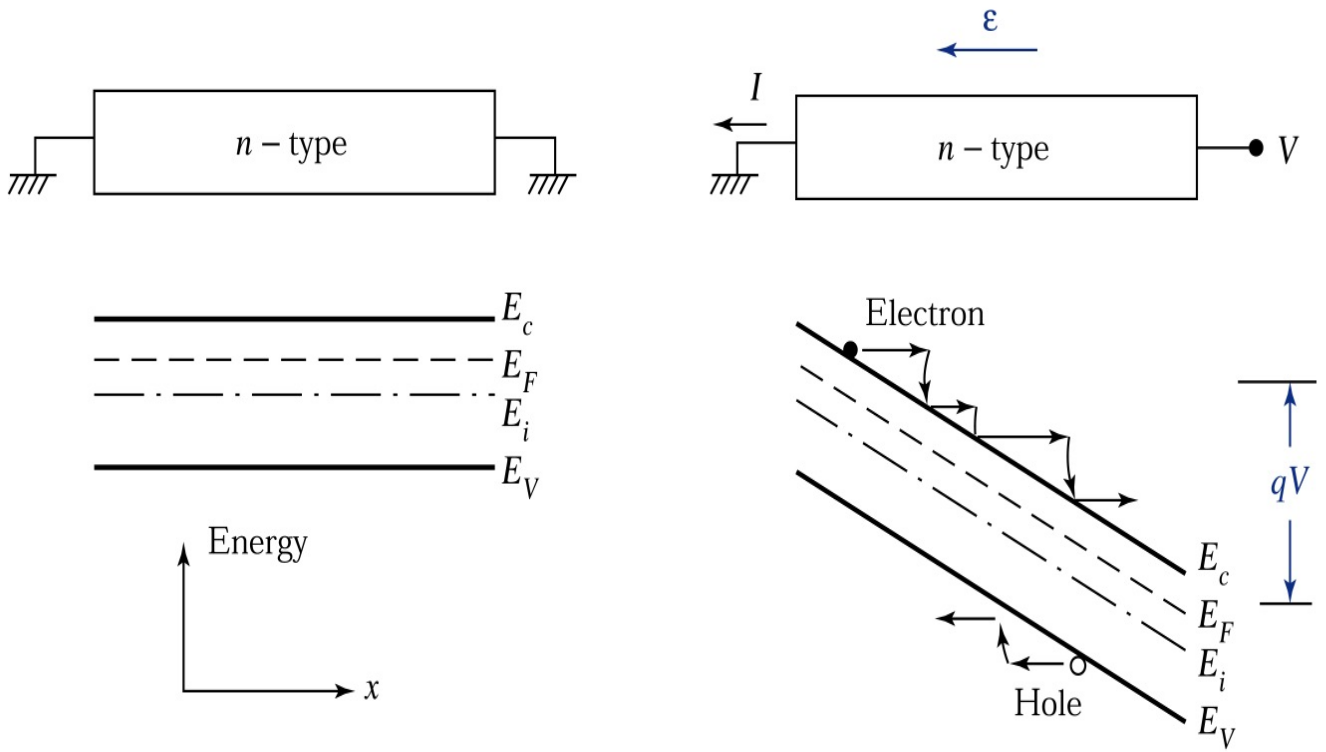
\includegraphics[width=0.8\linewidth]{Cuerpo/Ch_02/02_Campo_E.png}
	\caption{Efecto de un campo eléctrico externo en las bandas.}
	\label{Fig:02-03}
\end{figure}

Si $\psi$ es el \textit{potencial escalar eletroestático}, tenemos que:

\begin{equation}
	\Encal = \frac{1}{q} \derivadas{E_c}{x}= \frac{1}{q} \derivadas{E_i}{x}=- \derivadas{\psi}{x}
\end{equation}


%%%%%%%%%%%%%%%%%%%%%%%%%%%%%%%%%%%%%%%%%%%%%%%%%%%%%%%%%%%%%%%%%%%%%%%
%%%%%%%%%%%%%%%%%%%%%%%%%%%%%%%%%%%%%%%%%%%%%%%%%%%%%%%%%%%%%%%%%%%%%%%
%%%%%%%%%%%%%%%%%%%%%%%%%%%%%%%%%%%%%%%%%%%%%%%%%%%%%%%%%%%%%%%%%%%%%%%
%%%%%%%%%%%%%%%%%%%%%%%%  TEMA 2 %%%%%%%%%%%%%%%%%%%%%%%%%%%%%%%%%%
%%%%%%%%%%%%%%%%%%%%%%%%%%%%%%%%%%%%%%%%%%%%%%%%%%%%%%%%%%%%%%%%%%%%%%%
%%%%%%%%%%%%%%%%%%%%%%%%%%%%%%%%%%%%%%%%%%%%%%%%%%%%%%%%%%%%%%%%%%%%%%%
%%%%%%%%%%%%%%%%%%%%%%%%%%%%%%%%%%%%%%%%%%%%%%%%%%%%%%%%%%%%%%%%%%%%%%%


\section{Difusión}

La difusión es un proceso por el cual las partículas tienden a dispersarse o redistribuirse como restultado de su alta concentración en ciertas zonas del sólido o bajas concentraciones en otra zona a temperatura no nula. En este caso las partículas que sufren difusión son electrones y huecos, que harán aparecer corrientes de difusión.

\subsection{Corrientes de difusión}

La \textbf{ley de Flick} nos dice que las corrientes de difusión son directamente proporcionales a los gradientes de concetración de partículas, esto es:

\begin{equation}
	J_p|_{\text{difusión}} = -qD_p\nabla p \tquad
	J_n|_{\text{difusión}} =  qD_n\nabla n
\end{equation}
siendo $D_p$ y $D_n$ las llamadas \textit{constantes de difusión}, que dependen básicamente de dos términos: la velocidad media de nuestras partículas $v_{th}$ y el camino medio recorrido $\lambda$, tal que:

\begin{equation}
	D_n = v_{th} \lambda_{n} \qquad D_p = v_{th} \lambda_{p}
\end{equation}
En palabras: la capacidad de una partícula para difundirse depende tanto de qué tan rápido se mueve como de la distancia que recorre antes de cambiar de dirección. Para verlo mejor: imagina que una partícula se mueve en un entorno donde, cada cierto tiempo, choca y cambia de rumbo. Cuanto mayor sea su velocidad y mayor sea la distancia que recorre entre choques, más lejos llegará en promedio en un mismo intervalo de tiempo. Así, el producto de estos dos factores (velocidad y distancia entre colisiones) te da una medida de la eficacia con la que la partícula se dispersa en el medio. Esta difusión generará entonces la corriente de difusión de portadores tipo $n$ y tipo $p$.

\begin{equation}
	J_n |_{\text{difusion}} = qD_n \derivadas{n}{x} \qquad
	J_p |_{\text{difusion}} = -qD_p \derivadas{p}{x}
\end{equation}

\subsection{Relaciones de Einstein}

Las relación de Einstein para electrones nos permite relacionar el coeficiente de difusión y la movilidad para cada uno de los portadores con su carga y la temperatura del medio. La deducción de estas es trivial, ya que es consdierar que el semiconductor está en equlibrio y no degenerado

\begin{equation}
	J_n |_{\text{difusion}} +J_n |_{\text{arrastre}} = q\mu_n n \Encal + qD_n\derivadas{n}{x} = 0
\end{equation}
tal que

\begin{equation}
	n=n_i e^{(E_F-E_i)/kT} \Rightarrow \derivadas{n}{x} = - \frac{n_i}{kT} e^{(E_F-E_i)/kT} \derivadas{E_i}{x} = - \frac{n}{kT} \derivadas{E_i}{x} = - \frac{q}{kT} \Encal
\end{equation}
de lo cual se deduce

\begin{equation}
	J_n = (qn\Encal) \mu_n - qD_n \frac{q}{kT} n \Encal = 0
\end{equation}
resolviendo obtenemos la \textbf{relación de Einstein para los electrones}

\begin{equation}
	\frac{D_n}{\mu_n} = \frac{kT}{q}
\end{equation}
válida para semiconductores no degenerados tanto en equlibrio como fuera de él.



%%%%%%%%%%%%%%%%%%%%%%%%%%%%%%%%%%%%%%%%%%%%%%%%%%%%%%%%%%%%%%%%%%%%%%%
%%%%%%%%%%%%%%%%%%%%%%%%%%%%%%%%%%%%%%%%%%%%%%%%%%%%%%%%%%%%%%%%%%%%%%%
%%%%%%%%%%%%%%%%%%%%%%%%%%%%%%%%%%%%%%%%%%%%%%%%%%%%%%%%%%%%%%%%%%%%%%%
%%%%%%%%%%%%%%%%%%%%%%%%  TEMA 3 %%%%%%%%%%%%%%%%%%%%%%%%%%%%%%%%%%
%%%%%%%%%%%%%%%%%%%%%%%%%%%%%%%%%%%%%%%%%%%%%%%%%%%%%%%%%%%%%%%%%%%%%%%
%%%%%%%%%%%%%%%%%%%%%%%%%%%%%%%%%%%%%%%%%%%%%%%%%%%%%%%%%%%%%%%%%%%%%%%
%%%%%%%%%%%%%%%%%%%%%%%%%%%%%%%%%%%%%%%%%%%%%%%%%%%%%%%%%%%%%%%%%%%%%%%

\section{Procesos de generación y recombinación}

Cuando un semiconductor es perturbado de su estado de equilibrio, el semiconductor responde modificando el número de portadores que hay en el mismo. La recombinación-generación (denotada por RG o R-G) es el mecanismo con el que describimos el proceso por el cual un exceso o deficiencia de portadores se estabiliza (si la perturbación se mantiene en el tiempo) o es eliminada (si la perturbación es temporal). Dado que durante la perturbación el sistema está bajo condiciones de no equilibrio, muchas de los fenómenos que aparecen en el semiconductor no puedan ser descritos a través de los procesos RG.

\subsection{Introducción}

En un semiconductor definimos como \textbf{recombinación} al proceso por el cual electrones y huecos son aniquilados/destruidos, mientras que la \textbf{generación} es el proceso por el cual electrones y huecos son creados. Esta descripción así hecha es muy general, y por tanto varios tipos de procesos podrían incluirse en lo que llamamos RG. Generalmente se usan las gráficas de banda energética para describir visualmente cuales son los posibles procesos RG, aunque sea solo para entender su naturaleza. También se suele describir que papel tiene la energía y que tipo de energía se emite/absorbe en estos procesos.

\subsubsection{Procesos de recombinación}

Existen varios tipos de procesos de recombinación:

\begin{itemize}
	\item \textbf{Recombinación directa}. Es el tipo más simple de recombinación. En este hay una aniquilación directa entre un hueco en la banda de valencia y un electrón en la banda de conducción, en el que el electrón <<cae>> a la banda de valencia. Es un proceso típicamente radiativo, en el que el exceso de energía se convierte en un fotón de luz.

	\item \textbf{Recombinación de centro RG}. Recordemos que las impurezas generan niveles energéticos en la región del gap de energía. Los defectos cristalinos, particularmente las impurezas atómicas, pueden generar niveles energéticos en medio del gap. En este proceso de recombinación, los llamados centros RG con energía $E_T$ actúan como intermediarios. Existen varios tipos de recombinaciones de centro RG. En la primera de ellas tanto el electrón en la BC y el hueco en la BV se ven atraídos al mismo centro RG, aníquilándose. Otra posibilidad es que un portador salte a la banda contrario usando el centro RG como mediador. A este proceso se le llama \textit{recombinación termal}, ya que no es un proceso radiativo (no emite fotones), emitiendo calor, o, en su defecto, fonones. También existen recombinaciones de centro RG usando como centros RG los niveles energéticos de los dadores y aceptores (que recordemos están muy cerca de los niveles energéticos de las bandas), aunque no son tan comunes. Estos procesos son radiativos, pero poco probables, y se denominan \textit{recombinación a través de niveles profundos}. No son tan probables porque, a temperaturas ambientes, la probabilidad de que vuelvan a excitarse al nivel de la banda de conducción es altamente probable.

	\item \textbf{Recombinación Auger} En el proceso Auger lo que ocurre es que una recombinación directa/de centro RG ocurre simultáneamente con la colisión de dos portadores. Consecuentemente, estos portadores altamente energéticos se <<termalizan>>  (pierden energía en pasos pequeños mediante pequeñas colisiones con la red cristalina). La dispersión posterior del electrón que se lleva toda la energía sucede a través de diferentes pasos, como una <<escalera>>, lo cual sucede  porque la relajación del portador energético no es un proceso instantáneo, sino que sucede en varias etapas debido a la dispersión con fonones. Los fonones (vibraciones cuánticas de la red cristalina) tienen energías discretas, lo que significa que el portador pierde energía en múltiplos de estas energías fonónicas. En semiconductores típicos, los fonones ópticos tienen energías del orden de decenas de meV, por lo que un electrón altamente excitado no puede perder toda su energía de golpe, sino que la va cediendo en `saltos'' discretos al emitir fonones ópticos uno tras otro.

	\item \textbf{Recombinación superficial}:
\end{itemize}

\begin{Anotacion}
	\textcolor{red}{Importante colocar las imagenes}
\end{Anotacion}

\subsubsection{Procesos de generación}

Existen varios tipos de generación, uno por cada uno de los procesos de recombinación. Así pues, existe generación directa, la cual necesita energía térmica o electromagnética (a través de fotones); generación por centros RG (energía térmica), y en último lugar la generación a través de impactos ionizantes (proceso inverso a la recombinación Auger). En estos último, el par de portadores se genera como consecuencia del impacto de un portador con un átomo cristalino. La generación de portadores a través de impacto ionizante ocurre recurrentemente cuando hay regiones con un campo eléctrico $\Ecal$ muy alto, y es el responsable de los fenómenos de avalancha de las uniones $pn$.

\subsection{Consideraciones acerca los procesos RG}

Los procesos de recombinación y generación ocurren permanentemente, incluso en el equilibrio termodinámico, siendo el principal problema de los procesos RG el cálculo del ratio de producción de los diferentes procesos. Típicamente, uno solo necesita centrarse en el proceso principal (el que mayor ratio de producción tiene). En los semiconductores dopados no degenerados a una temperatura ambiente, uno esperea que los procesos dominantes sean procesos directos o de centro RG.

Conociendo la forma de las bandas de energía (más concretamente, cual es el valor de $k$ para el cual la energía de la banda de conducción es mínima) podremos dilucidad cual de los procesos es dominante: o de tipo directo o de centro RG. ¿Cómo? Pues es bien sencillo: los fotones, al ser partículas sin masa, son capaces de llevar muy poco momento, y por tanto las transiciones son casi verticales, es decir, solo son capaces de describir los semiconductores de tipo directo (mínimo BC y máximo de BV en $k=0$). Por otro lado, los fonones pueden trasmitir momentos y energía mucho mas grandes, por lo que son capaces de describir tanto los procesos en los semiconductores directos e indirectos, aunque en el caso de los directos no es un proceso dominante. Los procesos térmicos están relacionados con la recombinación de centro RG y los procesos fotónicos con la recombinación directa, y por tanto podemos diferenciar cuando uno y otro son dominantes.

\subsection{Recombinación directa en semiconductores de gap directo}

Definimos como $G$ ($R$) el número de pares electrones (huecos) generados $/\mathrm{cm}^3\mathrm{s}$. Estas tasas de recombinación y generación dependen en general del número de huecos y electrones que haya en el medio, por lo que en general:

\begin{equation}
	R = \beta np \tquad G = \alpha np
\end{equation}
Para un conductor en equilibrio termodinámico $G_{th}=R_{th}$ (siendo estas las tasas de generación/combinación en el equilibrio), manteniéndose $n$ y $p$ constantes. En el equilibrio  $R = G = \beta n_{n0}p_{n0}$.

\begin{figure}[h!] \centering
	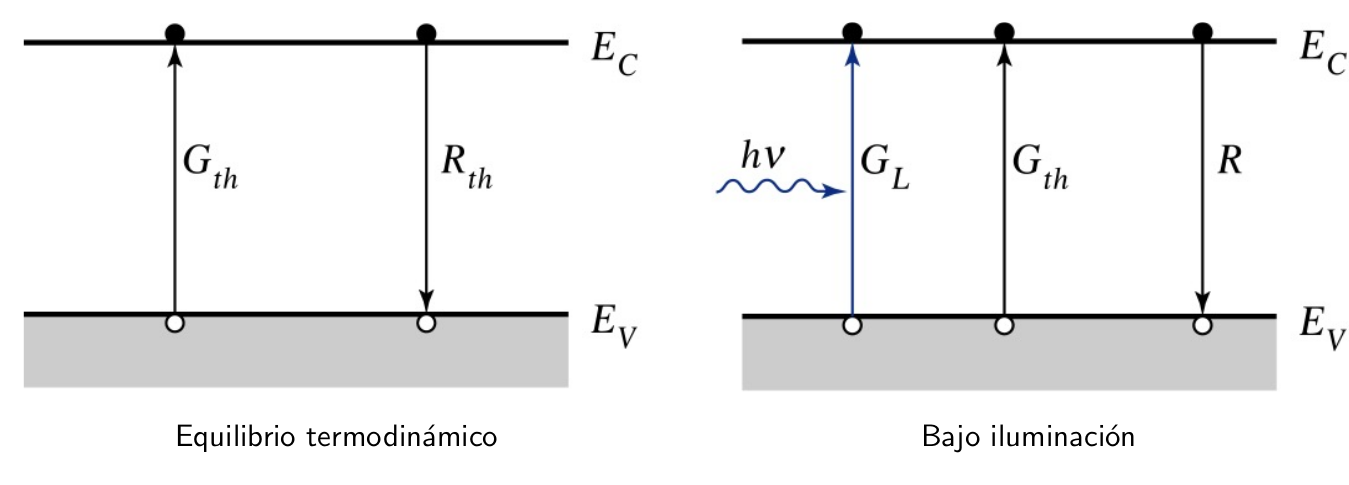
\includegraphics[width=0.9\linewidth]{Cuerpo/Ch_02/02_Luz.png}
	\caption{Procesos de generación y recombinación en equilibrio y sin luz.}
\end{figure}
Ahora bien, cuando iluminamos uno de estos semiconductores aumenta su generación en un término $G_L$, tal que ahora $G=G_L+G_{th}$. Consecuentemente tenemos que se incrementa en un número determinado el número de portadores en el semiconductor $\Delta n$ y $\Delta p$ ($\Delta n = \Delta p$, neutralidad de carga). Así pues tenemos que la tasa:


\begin{equation}
	\derivadas{p_n}{t} = G-R=G_L + G_{th} - R \tquad R = \beta n_n p_n = \beta (n_{n0}+\Delta n) (p_{n0}+\Delta p)
\end{equation}
Una vez llegamos al estado estacionario, podemos obtener entonces lo que llamamos el  \textit{ratio de recombinación} $U=R-G_{th}$, esto es:

\begin{equation}
	U = R-G_{th} = \beta (n_{n0}+p_{n0}+\Delta p)\Delta p
\end{equation}
Cuando tenemos $p_{n0}<<n_{n0}$ (bajo nivel de inyección tipo N), tenemos que:

\begin{equation}
	U = \beta n_{n0}\Delta p = \frac{p_n - p_{n0}}{\frac{1}{\beta n_{n0}}} =  \frac{p_n - p_{n0}}{\tau_p}
\end{equation}

\subsection{Recombinación indirecta en semiconductores de gap indirecto: procesos RG.}

\subsubsection{Definición de términos}

La estadística RG es el nombre que se le da a la caracterización matemática de los procesos de recombinación y generación. Dado que los procesos RG cambian las concentraciones de los portadores con el tiempo, la <<caracterización matemática>> de estos procesos no es más que la definición de las relaciones entre $\partial n / \partial t$ y $\partial p / \partial t$. Recordemos que los procesos RG lo que hacen es insertar una banda energética $E_T$ en la posición central del gap de bandas. Así pues definimos:

\begin{itemize}
	\item Variación de $n$ debida a procesos RG: $\eval{\parciales{n}{t}}_{RG}$.
	\item Variación de $p$ debida a procesos RG: $\eval{\parciales{p}{t}}_{RG}$.
	\item Número de centros RG llenos de electrones por $\mathrm{cm}^3$: $n_T$.
	\item Número de centros RG llenos de huecos por $\mathrm{cm}^3$ $p_T$
	\item Número total de centros RG por $\mathrm{cm}^3$: $N_T$
\end{itemize}
Es importante que quede muy claro que $\partial n / \partial t |_{RG}$ y $\partial p / \partial t|_{RG} $ son tasas netas, teniendo en cuenta tanto los procesos de recombinación como los procesos de generación. Cuando $\partial n / \partial t|_{RG}$ es negativo, la tasa de neta de electrones es negativa $R>G$; y si es postiva, la tasa de electrones es positiva $G>R$. La desingación de $|_{RG}$ no denota otra cosa que <<tasa de cambio producida por los procesos RG>>. Esto es importante, ya que pueden ocurrir otros procesos además de estos.

\begin{Anotacion}
	\textcolor{red}{Le llamo a $n_T$ centros ocuppados y a $p_T$ centros libres.}
\end{Anotacion}

\subsubsection{Obtención de las tasas de producción}

Existiendo 4 tipos de transiciones RG, que son:

\begin{itemize}
	\item \textbf{Captura de un electrón en un centro RG}. Se define $c_n$ como el \textit{coeficiente de captura de electrones} $(\text{cm}^3/s)$ con signo positivo. La tasa de captura de un electrón en un centro RG debe ser proporcional al número de centros disponibles para la captura $p_T$ y el número de electrones $n$.
	\item \textbf{Emisión de un electrón por un centro RG}.Se define $e_n$ como el \textit{coeficiente de emisión de electrones} $(\text{cm}^3/s)$ con signo positivo. La tasa de emisión de electrones debe ser proporcional al número de centros RG ocupados $n_T$.
	\item \textbf{Captura de un hueco en un centro de RG} (o un electrón de un RG cae a BV). Se define $c_p$ como el \textit{coeficiente de captura de huecos} $(\text{cm}^3/s)$ con signo positivo. La tasa de captura de un hueco en un centro RG debe ser proporcional al número de centros disponibles para la captura $n_T$ y el número de huecos $p$.
	\item \textbf{Emisión de un hueco por un centro de RG} (o un electrón de BV cae a RG). Se define $e_p$ como el \textit{coeficiente de emisión de electrones} $(\text{cm}^3/s)$ con signo positivo. La tasa de emisión de huecos debe ser proporcional al número de centros RG ocupados $pT$.
\end{itemize}
Una vez entendemos esto, es claro que las ecuaciones que rigen los procesos RG son (no pueden ser de otra forma)

\begin{equation}
	r_N = \eval{\parciales{n}{t}}_{RG} = e_n n_T - c_n n p_T \tquad r_P = 	\eval{\parciales{p}{t}}_{RG} = e_pp_T - c_p p n_T
\end{equation}

\subsection{Simplificaciones: balance detalado}

Existen varias simplificaciones. La más simple de todas es aquella en la que se aplica el \textbf{principio de balance detallado}. Este nos dice que bajo condiciones de equilibrio cada proceso fundamental y su inverso se autobalancean independientemente de cualquier otro proceso que peuda ocurrir en el interior del semiconductor. El equilibrio básicamente supone que el número de creación de huecos y electrones es cero, es decir:

\begin{equation}
	r_N = r_P = 0
\end{equation}
Luego tenemos que una de las constantes $e_{n,p}$ o $c_{n,p}$ se puede reescribir en función de la otra y en función del número de centros RG $n_T/p_T$ ocupados y el número de portadores $n$. El subíndice $0$ indica que estamos en el equlibrio:

\begin{equation}
	r_N = c_{n0} p_{T0} n_0 - e_{n0} n_{T0} = 0 \Rightarrow e_{n0} = \frac{c_{n0} p_{T0}n_0}{n_{T0}}
\end{equation}
\begin{equation}
	r_P = c_{p0} n_{T0} p_0 - e_{p0} p_{T0} = 0 \Rightarrow e_{p0} = \frac{c_{p0} n_{T0} p_0 }{p_{T0}}
\end{equation}
Si reescribimos $n_1=n_0p_{T0}/n_{T0}$ y $p_1=p_0n_{T0}/p_{T0}$ para simplificar las expresiones, tenemos que:

\begin{equation}
	e_{n0} = c_{n0} n_1 \tquad e_{p0} = c_{p0} p_1
\end{equation}
La simplificación se hace cuando asumimos que \textit{los coeficientes de emhiperbólicaisión y captura son aproximadamente los mismos en el equilibrio y fuera del equilibrio}, tal que

\begin{equation}
	e_n\approx e_{n0} = c_{n0} n_1 \approx c_n n_1 \tquad
	e_p\approx e_{p0} = c_{p0} p_1 \approx c_p p_1
\end{equation}
En el caso de que podamos asmir que los coeficientes de emisión y captura son parecidos a los coeficientes en el equilibrio:

\begin{equation}
	\begin{split}
		r_N = - \eval{\parciales{n}{t}}_{{RG}} & = c_n \parentesis{p_T n - n_T n_1} \\
		r_P =  \eval{\parciales{p}{t}}_{RG}    & = c_p \parentesis{n_T p - p_T p_1}
	\end{split}
\end{equation}
Reescribiendo $n_1$ y $p_1$:

\begin{equation}
	n_1 = \frac{p_{T0} n_0}{n_{T0}} = \parentesis{\frac{N_T-n_{T0}}{n_{T0}}} n_0 = \parentesis{\frac{N_T}{n_{T0}}-1} n_0
\end{equation}
\begin{equation}
	p_1 = \frac{n_{T0}p_0}{p_{T0}} = \parentesis{\frac{N_T-p_{T0}}{p_{T0}}} p_0 = \parentesis{\frac{N_T}{p_{T0}}-1} p_0
\end{equation}
Para un semiconductor no degenerado:

\begin{equation}
	n_0 = n_i e^{(E_F-E_i)/kT}
\end{equation}
Usando la definición de $n_T$ como

\begin{equation}
	\frac{n_{T0}}{N_T} = \frac{1}{1+g_T e^{(E_T-E_F)/kT}}
\end{equation}
Tomando $E'_T=E_T\pm\ln(g_T)$, donde $+$ es para un centro R-G aceptor y un signo $-$ para un centro R-G donador. Sustiyendo en $n_1$ y $p_1$:

\begin{equation}
	n_1 = \parentesis{\frac{N_T}{n_{T0}}-1} n_0 = n_i e^{(E_T'-E_i)/kT} \tquad
	p_1 = \parentesis{\frac{N_T}{p_{T0}}-1} p_0 = n_i e^{(E_i-E_T')/kT}
\end{equation}
Asumiendo que $E_T$ y $g_T$ son conocidos podemos calcular $n_1$ y $p_1$. Si $E_T'$ esa en el centro del gap, $n_1\approx p_1 \approx n_i$. Para la mayor parte de lo análisis que hacemos consideramos que el diapositiva se encuentra en estado estacionario o cuasi-estacionario (situación estable independiente del tiempo, distinto de equilibrio). En estado estacionario simplifica mucho el cálculo ya que si partimos que $n_T$ no cambia con en tiempo, y asumiendo que $n_T$ sólo puede cambiar mediante los centros de R-G:

\begin{equation}
	\parciales{n_T}{t} = - \eval{\parciales{n}{t}}_{R-G} + \eval{\parciales{p}{t}}_{R-G} = r_N - r_P = 0 \Rightarrow r_N = r_P
\end{equation}
La misma creación o aniquilación de huecos y electrones bajo las condiciones de estado estacionario, dejan fijo el valor de $n_T$ para valores dados $n$ y $p$. En concreto si igualamos el lado derecho de las ecuaciones:

\begin{equation}
	\begin{split}
		r_N = - \eval{\parciales{n}{t}}_{R-G} & = c_n (p_Tn - n_T n_1) \\
		r_P = - \eval{\parciales{p}{t}}_{R-G} & = c_p (n_Tn - p_T p_1)
	\end{split}
\end{equation}
Teniendo en cuenta que $p_T=N_T-n_T$, si despejamos $n_T$ obtenemos:

\begin{equation}
	n_T = \frac{c_n N_T n + c_p N_T p_1}{c_n(n+n_1)+c_p(p+p_1)}
\end{equation}
Obtenemos

\begin{equation}
	R=r_N=r_P = \frac{np-n_i^2}{\frac{1}{c_p N_T} (n+n_1) + \frac{1}{c_nN_T}\parentesis{p+p_1}} =
	\frac{np-n_i^2}{\tau_p(n+n_1)+\tau_n(p+p_1)}
\end{equation}
donde $\tau_n$ y $\tau_p$ son la vida mediade los electrones y huecos minoritarios. El símbolo $R$ identificala tasa neta de recombinación en estado estacionario. Vamos a realizar ahora dos simplificaciones para obtener un resultado más sencillo de la recombinación para los casos de:

\begin{itemize}
	\item Bajo nivel de inyección.
	\item Semiconductor vacío de portadores.
\end{itemize}

\subsubsection{Bajo nivel de inyección}

Vamos ahora a realizar otra simplificación para obtener un resultado más sencillo de la recombinación para el caso de \textbf{bajo nivel de inyección (BNI)}, que implica:

\begin{equation}
	\left.
	\begin{matrix}
		\Delta n = n - n_0 \\
		\Delta p = p - p_0
	\end{matrix}
	\right\rbrace
	\text{BNI} \rightarrow
	\left\lbrace
	\begin{matrix}
		\Delta n \ll n_0; \ \text{Tipo N:} \ n \approx n_0 \\
		\Delta p \ll p_0; \ \text{Tipo P:} \ p \approx p_0
	\end{matrix}
	\right.
\end{equation}
Asumiendo las sigueintes consideraciones:

\begin{itemize}
	\item Bajo nivel de inyección.
	\item Los centros RG dominantes introducen un nivel de energía $E_T$ próximo al centro del gap. Tenemso que $n_1\approx p_1\approx n_i$.
	\item La concentración de centros RG es muy baja lo que implica que $\Delta n \approx \Delta p$.
	\item Consideramos que $E_F'$ está próximo a la mitad del gap con lo que podemos aproximar $n_1\approx p_1\approx n_i$.
	\item Las vidas medias $\tau_n$ y $\tau_p$, no se diferencian en más que unos cuantos órdenes de magnitud.
	\item Por último: $n=n_0 + \Delta n$ y $p=p_0+\Delta p$; $\Delta n \approx \Delta p$ y $n_1 \approx p_1 \approx n_i$.
\end{itemize}
Obtenemos el siguiente valor como \textit{tasa de recombinación}:
\begin{equation}
	R = \frac{(n_0+\Delta n)(p_0 + \Delta p)-n_i^2}{\tau_p(n_0+\Delta n + n_1)+\tau_n (p_0 + \Delta p + p_1)}
\end{equation}
Veamos cual es este valor de $R$ para los tipo $p$ y tipo $n$:
\begin{itemize}
	\item Para un semicondutor tipo N podemos consdierar que $n_0\gg p_0$ y $n_0 p_0 = n_i^2$, así:

	      \begin{equation}
		      \left.
		      \begin{split}
			      n_0 \gg & p_0 + \Delta p + n_i \\
			      \tau_n  & \approx \tau_p
		      \end{split}
		      \right\rbrace \rightarrow \tau_p n_0 \gg \tau_n (p_0 + \Delta p + n_i)
	      \end{equation}
	      Teniendo en cuenta que $n_0\Delta p\gg p_0\Delta n$ y que $n_0 \Delta p \gg (\Delta p)^2$:

	      \begin{equation}
		      R \approx \frac{n_0\Delta p}{\tau_p n_0} = \frac{\Delta p}{\tau_p}
	      \end{equation}
	\item Para un semiconductor tipo P, haciendo las mismas consideraciones

	      \begin{equation}
		      \left.
		      \begin{split}
			      p_0 \gg & n_0 + \Delta n + n_i \\
			      \tau_n  & \approx \tau_p
		      \end{split}
		      \right\rbrace \rightarrow \tau_n p_0 \gg \tau_p (n_0 + \Delta n + n_i)
	      \end{equation}
	      Teniendo en cuenta que $p_0\Delta n\gg n_0\Delta p$ y que $p_0 \Delta n \gg (\Delta n)^2$:

	      \begin{equation}
		      R \approx \frac{p_0\Delta n}{\tau_n p_0} = \frac{\Delta n}{\tau_n}
	      \end{equation}
\end{itemize}

\subsubsection{Semiconductor vacío de portadores}

La región vacía de portadores se define como un volumen del semiconductor donde consideramos que el semiconductor está vacío de portadores:

\begin{equation}
	\left. \begin{matrix}
		n \ll n_i \\
		p \ll n_i
	\end{matrix} \right\rbrace np \ll n_1 p_1 = n_i^2
\end{equation}
En este caso:

\begin{equation}
	R = \frac{np-n_i^2}{\tau_p (n+n_1)+\tau_n(p+p_1)} = - \frac{n_i}{\tau_g}
\end{equation}
donde $\tau_g = \tau_p (n_1/n_i) + \tau_n (p_1 / n_i)$ es el tiempo medio de generación. El signo menos indica que dentro de la región vacía tiene lugar una generación neta de portadores. Si $E_T'=E_i$ entonces $\tau_g=\tau_p+\tau_n$.

\subsection{Recombinación Auger}

Como sabemos, la recombinación Auger ocurre cuando se transfiere energía y momento de una recombinación de un par de portadores a un tercer portador, lo que hace que adquiera una energía y momento elevados. Esta energía y momento elevados se dispersan al medio a través de la dispersión con la red cristalina, por ejemplo en forma de fonones. Esta dispersión en forma de fonones hace que pierda energía de manera discreta, lo cual tiene sentido si pensamos que está emitiendo cuantos de energía (fonones). Este tipo de procesos es importante a alto dopado/alto nivel de inyección:

\begin{equation}
	R_{\text{Auger}} = \beta n^2 p \tquad R_{\text{Auger}} = \beta p^2 n
\end{equation}
La constante $\beta$ depende fuertemente de la tempeartura. 

\begin{Anotacion}
	\textcolor{red}{¿Por qué es un proceso que cobra importancia a alto nivel de inyección y dopado?¿Qué significa alto nivel de inyección?¿Esta $\beta$ coincide con la $\beta$ del proceso de fotogeneración?}
\end{Anotacion}

\subsection{Recombinación superficial}

La recombinación superficial es la recombinación que ocurre cerca de la superficie debido a la aparición de estados energéticos que se pueden usar como centros RG. Con bajo nivel de inyección, la concentración superficial es similar a la concentración en volumen. Así, la tasa de recombinación por unidad de área y tiempo es:

\begin{equation}
	U  \simeq v_{th} \sigma_p N_{st} (p_s-p_{n0})
\end{equation}
donde $p_s$ es la \textit{concetración de huecos en la superficie}, $N_{st}$ la \textit{densidad de centros recombinadores por unidad de área en la superficie}, $v_{th}$ la \textit{velcoidad térmica} y $\sigma_p$ es el \textit{coeficiente de captura de huecos}. A baja inyección definimos el coeficiente de la siguiente manera:

\begin{equation}
	S_{lr} \equiv v_{th} \sigma_p N_{st}
\end{equation}

\begin{Anotacion}
	\textcolor{red}{¿Cómo aparecen estros centros RG?¿Por qué?¿No fallan las unidades?¿Por qué esa aproximación a bajo nivel de inyección?}
\end{Anotacion}


%%%%%%%%%%%%%%%%%%%%%%%%%%%%%%%%%%%%%%%%%%%%%%%%%%%%%%%%%%%%%%%%%%%%%%
%%%%%%%%%%%%%%%%%%%%%%%%%%%%%%%%%%%%%%%%%%%%%%%%%%%%%%%%%%%%%%%%%%%%%
%%%%%%%%%%%%%%%%%%%%%%%%%%%%%%%%%%%%%%%%%%%%%%%%%%%%%%%%%%%%%%%%%%%%
%%%%%%%%%%%%%%%%%%%%%%%% TEMA 4 %%%%%%%%%%%%%%%%%%%%%%%%%%%%%%%%%%%
%%%%%%%%%%%%%%%%%%%%%%%%%%%%%%%%%%%%%%%%%%%%%%%%%%%%%%%%%%%%%%%%%%%%
%%%%%%%%%%%%%%%%%%%%%%%%%%%%%%%%%%%%%%%%%%%%%%%%%%%%%%%%%%%%%%%%%%%%%
%%%%%%%%%%%%%%%%%%%%%%%%%%%%%%%%%%%%%%%%%%%%%%%%%%%%%%%%%%%%%%%%%%%%%%

\section{Ecuaciones de continuidad}


\subsection{Introducción}

La tasa de cambio de portadores viene dada entonces por la suma de todas las tasas de cambio estudiadas hasta el momento: arrastre, difusión, recombinación-generación...

\begin{equation}
	\parciales{n}{t} = \eval{\parciales{n}{t}}_{\text{Arrastre}}+\eval{\parciales{n}{t}}_{\text{Difusion}}+\eval{\parciales{n}{t}}_{\text{RG}}+\eval{\parciales{n}{t}}_{\text{Otros}}
\end{equation}
\begin{equation}
	\parciales{p}{t} = \eval{\parciales{p}{t}}_{\text{Arrastre}}+\eval{\parciales{p}{t}}_{\text{Difusion}}+\eval{\parciales{p}{t}}_{\text{RG}}+\eval{\parciales{p}{t}}_{\text{Otros}}
\end{equation}
Ahora solo tenemos que sustituir las expresiones vistas. Recordemos que las ecuacioens de continuidad nos dicen que la tasa de cambio por unidad de volumen es igual a la divergencia de la corriente. Así pues: 

\begin{itemize}
	\item Las ecuaciones de \textit{arrastre} nos dicen que:
	\begin{equation}
		\eval{\parciales{n}{t}}_{\text{Arrastre}} = \frac{1}{q} \div  \Jn_n |_{\text{Arrastre}} = \frac{1}{q} \div \parentesis{qn\mu_n \Encal}
	\end{equation}
	\begin{equation}
		\eval{\parciales{p}{t}}_{\text{Arrastre}} = \frac{1}{q} \div  \Jn_p|_{\text{Arrastre}} = \frac{1}{q} \div \parentesis{qp\mu_p \Encal}
	\end{equation}
	\item Las ecuaciones de \textit{difusión} nos dicen que:
	\begin{equation}
		\eval{\parciales{n}{t}}_{\text{Difusonn}} = \frac{1}{q} \div  \Jn_n|_{\text{Difusion}} = \frac{1}{q} \div \parentesis{D_n \grad n}
	\end{equation}
	\begin{equation}
		\eval{\parciales{p}{t}}_{\text{Difusonn}} = - \frac{1}{q} \div  \Jn_p|_{\text{Difusion}} = - \frac{1}{q} \div \parentesis{D_p\grad p}
	\end{equation}
	\item Las ecuaciones de \textit{Recombinación-Generación} nos dicen que:
	\begin{equation}
		\eval{\parciales{n}{t}}_{\text{Arrastre}} = G_n - R_n
	\end{equation}
	\begin{equation}
		\eval{\parciales{p}{t}}_{\text{Arrastre}} = G_p - R_p
	\end{equation}
\end{itemize}
De lo que se deduce que las \textbf{ecuaciones de continuidad} son

\begin{equation}
	n =\div \parentesis{qn\mu_n \Encal +  D_n \grad n  } + G_n - R_n
\end{equation}
\begin{equation}
	p = \div \parentesis{qp\mu_p \Encal +  D_p \grad p  } + G_p - R_p
\end{equation}
Y si consdieramos la movilidad como la difusión constantes en el semiconductor:

\begin{equation}
	n = \mu_n (\grad n) \cdot \Encal + \mu_n n \div \Encal + D_n \grad n + G_n - R_n
\end{equation}
\begin{equation}
	p = \mu_p (\grad p) \cdot \Encal + \mu_p p \div \Encal - D_p \grad n + G_p - R_p
\end{equation}
Esta seria la \textit{expresión más general posible}, lógicamente ahora habría que hacer diferentes aproximaciones en función del caso.

%%%%%%%%%%%%%%%%%%%%%%%%%%%%%%%%%%%%%%%%%%%%%%%%%%%%%%%%%%%%%%%%%%%%%%%
%%%%%%%%%%%%%%%%%%%%%%%%%%%%%%%%%%%%%%%%%%%%%%%%%%%%%%%%%%%%%%%%%%%%%%%
%%%%%%%%%%%%%%%%%%%%%%%%%%%%%%%%%%%%%%%%%%%%%%%%%%%%%%%%%%%%%%%%%%%%%%%
%%%%%%%%%%%%%%%%%%%%%%%%  TEMA 5 %%%%%%%%%%%%%%%%%%%%%%%%%%%%%%%%%%
%%%%%%%%%%%%%%%%%%%%%%%%%%%%%%%%%%%%%%%%%%%%%%%%%%%%%%%%%%%%%%%%%%%%%%%
%%%%%%%%%%%%%%%%%%%%%%%%%%%%%%%%%%%%%%%%%%%%%%%%%%%%%%%%%%%%%%%%%%%%%%%
%%%%%%%%%%%%%%%%%%%%%%%%%%%%%%%%%%%%%%%%%%%%%%%%%%%%%%%%%%%%%%%%%%%%%%%


\section{Pseudoniveles de Fermi}

Los pseudoniveles de Fermi se introducen de manera que podemos reexpresar las concentracioens, sustituyendo $E_F\rightarrow E_{Fn},E_{Fp}$, esto es, \textit{pseudonivel de Fermi para electroens y para huecos}:

\begin{equation}
	n=N_C e^{(E_{Fn}-E_c)/kT} \tquad 
	p=N_V e^{(E_{v}-E_{Fp})/kT}
\end{equation}
Estos son válidos cuando los electrones y huecos están en equilibrio térmico en sus bandas, y el tiempo de recombinación es mayor que el tiempo qeu necesitan parar que alcancen el equlibrio dentro de las bandas.

\begin{Anotacion}
	\textcolor{red}{¿Por qué se introducen, qué ganamos?¿Es fenomenológico?}
\end{Anotacion}



%%%%%%%%%%%%%%%%%%%%%%%%%%%%%%%%%%%%%%%%%%%%%%%%%%%%%%%%%%%%%%%%%%%%%%%
%%%%%%%%%%%%%%%%%%%%%%%%%%%%%%%%%%%%%%%%%%%%%%%%%%%%%%%%%%%%%%%%%%%%%%%
%%%%%%%%%%%%%%%%%%%%%%%%%%%%%%%%%%%%%%%%%%%%%%%%%%%%%%%%%%%%%%%%%%%%%%%
%%%%%%%%%%%%%%%%%%%%%%%%  TEMA 6 %%%%%%%%%%%%%%%%%%%%%%%%%%%%%%%%%%
%%%%%%%%%%%%%%%%%%%%%%%%%%%%%%%%%%%%%%%%%%%%%%%%%%%%%%%%%%%%%%%%%%%%%%%
%%%%%%%%%%%%%%%%%%%%%%%%%%%%%%%%%%%%%%%%%%%%%%%%%%%%%%%%%%%%%%%%%%%%%%%
%%%%%%%%%%%%%%%%%%%%%%%%%%%%%%%%%%%%%%%%%%%%%%%%%%%%%%%%%%%%%%%%%%%%%%%


\section{Otros fenómenos de transporte}

Exissten otros procesos que provocan corrientes en los portadores. Estas son:

\subsection{Emisión termoiónica}

En este proceso los electrones son emitidos al vacío.

\begin{Anotacion}
	\textcolor{red}{¿Qué es el vacío?}
\end{Anotacion}

\subsection{Transporte túnel}

Existe la posibilidad no nula de que los electrones traspasen una barrera de potencial a través del efecto túnel. Este proceso es importante cuando hay un hueco entre dos semiconductores (que se representa como un potencial constante y alto respecto el nivel de Fermi). 


\subsection{Efectos a campos altos}

Al aumentar el campo eléctrico lo suficiente ($\sim 5 \times 10^3$ V/m) la velocidad se satura. Sin embargo, cuando nuestro semiconductor tiene más de un mínimo local en la banda de valencia, puede ocurrir que $\Ecal$ sea tan grande que haga que pasen del mínimo absoluto a este mínimo local, lo que haría que la masa efectiva cambiase (al tener difernete Curvatura) lo que puede ocasionar que no satura, si no que disminuya o aumente la velocidad.



\newpage


%%%%%%%%%%%%%%%%%%%%%%%%%%%%%%%%%%%%%%%%%%%%%%%%%%%%%%%%%%%%%%%%%%%%%%%
%%%%%%%%%%%%%%%%%%%%%%%%%%%%%%%%%%%%%%%%%%%%%%%%%%%%%%%%%%%%%%%%%%%%%%%
%%%%%%%%%%%%%%%%%%%%%%%%%%%%%%%%%%%%%%%%%%%%%%%%%%%%%%%%%%%%%%%%%%%%%%%
%%%%%%%%%%%%%%%%%%%%%%%%  EJERCICIOS %%%%%%%%%%%%%%%%%%%%%%%%%%%%%%%%%%
%%%%%%%%%%%%%%%%%%%%%%%%%%%%%%%%%%%%%%%%%%%%%%%%%%%%%%%%%%%%%%%%%%%%%%%
%%%%%%%%%%%%%%%%%%%%%%%%%%%%%%%%%%%%%%%%%%%%%%%%%%%%%%%%%%%%%%%%%%%%%%%
%%%%%%%%%%%%%%%%%%%%%%%%%%%%%%%%%%%%%%%%%%%%%%%%%%%%%%%%%%%%%%%%%%%%%%%


\section{Ejercicios}

\subsection{Ejercicio 1}

Cuestiones sobre la resistividad y movilidad:
\begin{enumerate}[label=\alph*)]
	\item La resistividad de un material tipo N es por lo regular más pequeña que la resistividad de un material tipo P de dopado comparable, explica por qué suele ocurrir esto. Calcula la resistividad del Si si se dopa con fósforo con una concentración de \( 10^{17} \) cm\(^{-3}\). Repite el cálculo para el caso en que dopemos con aluminio con la misma concentración y calcular la corriente de arrastre en ambos casos considerando un campo eléctrico de \( 10^5 \) V/cm.

	\item Calcula la densidad de impurezas necesarias para tener un cristal de Si tipo P con resistividad 0.1 \(\Omega\cdot\)cm. ¿Qué proporción hay de átomos de impureza sobre el número de átomos de Si?
		  (DATO: Constante de red del Si \( a_0 = 5.431 \) Å). Si suponemos que el semiconductor es no degenerado, ¿cuánto vale \( D_p \)?
\end{enumerate}


\rule{\textwidth}{0.1pt} \\[2pt]

\begin{enumerate}[label=\alph*)]
	\item La diferentencia radica en la masa efectiva, que se expresa en la movilidad:
		  \begin{equation}
			  \rho = \frac{1}{q(n\mu_n + p \mu_)}
		  \end{equation}
		  Cuando $\mu_n>\mu_p \Rightarrow \rho_n < \rho_p$. Y esto siempre ocurre. Las movilidades dependen de la temperatura y la cantidad que esté dopado, por lo que puede ser diferente. Para un semiconductor dopado tipo $N$:

		  \begin{equation}
			  \rho_N = \frac{1}{qn{\mu_n}} = \frac{1}{1.6\cdot 10^{19} \cdot 10^{17}\cdot 1350}= 0.0463 \Omega \cm
		  \end{equation}
		  Y para un tipo $P$:
		  \begin{equation}
			  \rho_N = \frac{1}{1.6\cdot 10^{19} \cdot 10^{17}\cdot 480} = 0.13 \Omega \cm
		  \end{equation}
		  (valores de movilidad sacados de la Wikipedia). Ahora podemos calucular la corriente de arrastre (usamos que $J=qnN\epsilon$, donde $\epsilon = 10^5$ eV)
		  \begin{equation}
			  J_N =  2.16 \cdot 10^6  A\cm^{-2}  \tquad J_p = 7.68 \cdot 10^3  A\cm^{-2}
		  \end{equation}
	\item Ahora lo que hacemos es considerar que el número de impurezas es igual al número de huecos (están todas completamente ionizadas). Lo que nos queda entonces es:
		  \begin{equation}
			  N_A = \frac{1}{q\rho \mu_p } = \frac{1}{1.6\cdot 10^{19} \cdot 0.1 \cdot 480} = 1.3 \cdot 10^{17} \cm^{-3}
		  \end{equation}
		  Podemos calcular con $a_0$ el númerode átomos de silicio por unidad de volumen:

		  \begin{equation}
			  N_{Si} = 5 \cdot 10^{22} \text{at} \cm^{-3}
		  \end{equation}
		  Y solo tenemos, para calcular la proporción:

		  \begin{equation}
			  \frac{N_A}{N_{Si}} = 2.6 \cdot 10^{-6} = 2.6 \ \text{ppm}
		  \end{equation}
		  Para acabar necesitamos calcular la relación de Eistein (solo usable en semicdonductores no degenerados). Así tenemos que

		  \begin{equation}
			  D_p = \frac{kT}{q} \mu_p = 12.4 \cm^2 / s
		  \end{equation}
\end{enumerate}

\rule{\textwidth}{0.1pt} \\[2pt]

\subsection{Ejercicio 2}

Responde a las siguientes cuestiones:
\begin{enumerate}
	\item[a)] Calcular la resistividad del GaAs intrínseco a temperatura ambiente ($\mu_n = 9200$ cm$^2$/Vs, $\mu_p = 320$ cm$^2$/Vs).

	\item[b)] La movilidad de los electrones en el silicio es $\mu_n = 1300$ cm$^2$/Vs a temperatura ambiente. Si asumimos que la movilidad está limitada principalmente por la dispersión con la red cristalina, calcular la movilidad a $T= 150$ K.

	\item[c)] Dos mecanismos de dispersión tienen lugar en un semiconductor. Si sólo el primer de los mecanismos está presente la movilidad es de 250 cm$^2$/Vs. Si sólo el segundo de los mecanismos está presente la movilidad es de 650 cm$^2$/Vs. Calcular la movilidad cuando los dos mecanismos están presentes.
\end{enumerate}

\rule{\textwidth}{0.1pt} \\[2pt]

\begin{enumerate}[label=\alph*)]
	\item Para calcular la resistividad usamos la fórmula:
	\begin{equation}
		\rho = \frac{1}{q(\mu_p p + \mu_n n )}
	\end{equation}
	Donde solo tenemos que sustituir $n,p\rightarrow n_i$. Calculamos usando que $n_i= 2.25\times 10^6 \cm^{-3}$ de lo que se deduce que:
	\begin{equation}
	\rho =4.33\cdot 10^9 \ \Omega \cm
	\end{equation}
	\textcolor{Blue}{Creo que hay algo mal en el resultado numérico aunque la ecuación está bien. Podría dar entorno a 2.5 por diez a la diez, más o menos.}
	\item No conocemos la fórmula explícita, pero śi que sabemos que $\mu_{\text{impurezas}}\propto T^{-3/2}$ (red cristalina es igual a dispersión por fonones). Por tanto podemos calcular:
	\begin{equation}
		\frac{\mu_{\text{imp}} (T=150K)}{\mu_{\text{imp}}(T=300K)} = \parentesis{\frac{150}{300}}^{-3/2}		
	\end{equation}
	De lo que obtenemos:
	\begin{equation}
		\mu_{\text{imp}} (T=150K) = 3677 \ \cm^2 / \text{Vs}
	\end{equation}
	\item Tenemos que usar la \textit{regla mathiessen}:
	\begin{equation}
		\frac{1}{\mu} = \frac{1}{\mu_{1}}+\frac{1}{\mu_{2}} 
	\end{equation}
	De lo que obtenemos:		
	\begin{equation}
		\mu = 180.55 \ \cm^2 / \text{Vs} 
	\end{equation}
\end{enumerate}

\rule{\textwidth}{0.1pt} \\[2pt]

\subsection{Ejercicio 3}
Obtener las concentraciones de electrones y huecos, movilidades y resistividades de muestras de silicio a \(300 K\) para las siguientes concentraciones de impurezas:
\begin{itemize}
	\item[(a)] \(1 \times 10^{15}\) átomos/cm$^3$ de boro.
	\item[(b)] \(1 \times 10^{16}\) átomos/cm$^3$ de boro y \(1.5 \times 10^{16}\) átomos/cm$^3$ de arsénico.
	\item[(c)] \(5 \times 10^{15}\) átomos/cm$^3$ de boro, \(10^{17}\) átomos/cm$^3$ de arsénico y \(10^{17}\) átomos/cm$^3$ de galio.
\end{itemize}
Considerar que, las movilidades para portadores mayoritarios:
\begin{equation}
	\mu_n (N) = 65  + \frac{1265}{1+\parentesis{\frac{N}{8.5\times 10^{16}}}^{0.72}} \qquad 
	\mu_p (N) = 48  + \frac{447}{1+\parentesis{\frac{N}{6.3\times 10^{16}}}^{0.76}}
\end{equation}
Para portadores minoritarios:
\begin{equation}
	\mu_n (N) = 232  + \frac{1180}{1+\parentesis{\frac{N}{8\times 10^{16}}}^{0.9}} \qquad 
	\mu_p (N) = 130  + \frac{370}{1+\parentesis{\frac{N}{8\times 10^{17}}}^{1.25}}
\end{equation}


\rule{\textwidth}{0.1pt} \\[2pt]

Primero tenemos que evaluar si son dadores/aceptores, calcular $n$ y $p$, luego evaluar las fórmulas para portadores mayoritarios y minoritarios, y finalmente la resistividad. \textcolor{red}{Tengo que cambiar los datos, ya que $N=N_A+N_D$, teniendo que calcular n y p de una manera difernte a $p=N_D$.}  Para calcular $n$ y $p$:
\begin{enumerate}[label=\alph*)]
	\item El Boro es un átomo aceptor, por lo que tendremos como dato $N_A=10^{15} \ $átomos/$\cm^3$. Ahora calculamos, usando que $n_i=1.18\times 10^{10}$:   
	\begin{equation}
		p = N_A = 10^{15} \qquad n = \frac{n_i^2}{p} =1.39 \cdot 10^5 \cm^-3
	\end{equation}
	Calculamos las movilidades, usando la mayoritaria para los huecos y la minoritaria para los electrones:
	\begin{equation}
		\mu_p=4.77\cdot 10^2  \ \cm^2 /  \text{V s} \qquad 
		\mu_n=1.39 \cdot 10^3 \ \cm^2 /  \text{V s}
	\end{equation}
	La resistividad $\rho$ se calcula ahora fácilmente:
	\begin{equation}
		\rho = \frac{1}{e(\mu_n n + \mu_pp)} \rightarrow 
		\rho = 13.1 \ \Omega \cm
	\end{equation}

	\item El Arsénico es un átomo dador, por lo que tendremos como dato $N_{D\text{eff}}=5 \times 10^{15} \ $átomos/$\cm^3$, que se deduce de:
	\begin{equation}
		N_{D\text{eff}} = N_{\text{As}} - N_{\text{B}} = 5 \times 10^{15}
	\end{equation}
	Ahora calculamos, usando que $n_i=1.18\times 10^{10}$:   
	\begin{equation}
		n = N_{D\text{eff}} = 10^{15} \qquad p = \frac{n_i^2}{n} = 2.78 \cdot 10^4 \cm^-3
	\end{equation}
	Calculamos las movilidades, usando la mayoritaria para los electrones y la minoritaria para los huecos:
	\begin{equation}
		\mu_n=9.60 \cdot 10^2  \ \cm^2 /  \text{V s} \qquad 
		\mu_p=4.89 \cdot 10^2  \ \cm^2 /  \text{V s}
	\end{equation}
	La resistividad $\rho$ se calcula ahora fácilmente:
	\begin{equation}
		\rho = \frac{1}{e(\mu_n n + \mu_pp)} \rightarrow \rho = 1.3 \ \Omega \cm
	\end{equation}
	ESTA TODO MAL.
	\item El Galio es un átomo aceptor, por lo que tendremos como dato $N_{A\text{eff}}=5 \times 10^{15} \ $átomos/$\cm^3$, que se deduce de:
	\begin{equation}
		N_{A\text{eff}} = N_{\text{Ga}} + N_{\text{B}} - N_{\text{As}} =  2.78 \cdot 10^4 \ \cm^{-3}
	\end{equation}
	Ahora calculamos, usando que $n_i=1.18\times 10^{10}$:   
	\begin{equation}
		p = N_{A\text{eff}} = 5 \times 10^{15} \qquad p = \frac{n_i^2}{n} = 3e+04 \cm^-3
	\end{equation}
	Calculamos las movilidades, usando la mayoritaria para los huecos y la minoritaria para los electrones:
	\begin{equation}
		\mu_p=4.38 \cdot 10^{2}  \ \cm^2 /  \text{V s} \qquad 
		\mu_n=1.18 \cdot 10^{3} \ \cm^2 /  \text{V s}
	\end{equation}
	La resistividad $\rho$ se calcula ahora fácilmente:
	\begin{equation}
		\rho = \frac{1}{e(\mu_n n + \mu_pp)} \rightarrow 
		\rho = 2.85 \ \Omega \cm
	\end{equation}
	ESTA TODO MAL.
\end{enumerate}

\rule{\textwidth}{0.1pt} \\[2pt]

\subsection{Ejercicio 4}

\begin{itemize}
\item[(a)] Una muestra de silicio intrínseco es dopada desde un lateral con donadores de tal forma que:
\[
	N_D = N_0 \exp(-ax).
\]
Suponiendo condiciones de equilibrio y que \(N_D \gg n_i\), encontrar la expresión del campo eléctrico interno \(E(x)\). Evaluar \(E(x)\) para \(a = 10^{-6} \, \text{m}^{-1}\).
\item[(b)] Si ahora el perfil de dopado es:
\[
	N_D(x) = N_0+(N_L-N_0)(x/L),
\]
obtener una expresión para el campo eléctrico en un plano \(x\) dentro del dispositivo, considerando constantes el coeficiente de difusión y la movilidad. ¿Cuál es la expresión de la diferencia de potencial entre las superficies frontal y trasera de la muestra si la muestra es de longitud \(L\)? Consideraremos condiciones de equilibrio térmico y eléctrico.
\end{itemize}


\rule{\textwidth}{0.1pt} \\[2pt]

\begin{enumerate}[label=\alph*)]
	\item Nos dicen que $N_D=N_0 \exp(-ax)$, y queremos calcular $E(x)$. Dependerá del nivel de profundidad que quieres darle al ejercicio. Suponemos, al no dar datos de los procesos recombinación-generación, que estamos en el \textit{modelo de arrastre-difusión}. Así pues, tenemos que:
	\begin{equation}
		\parciales{n}{t} = \div \Jn = 0 \rightarrow \div (\Jn_{\arr}+\Jn_{\diff}) = 0 \rightarrow J_{\arr}+J_{\diff} = 0
	\end{equation}
	tal que (pasamos de vectorial a escalar)
	\begin{equation}
		J_{\arr}+J_{\diff} = 0 \rightarrow q \mu_n n \Ecal + q D_n \derivadas{n}{x} = 0 \rightarrow \Ecal = - \frac{D_n}{\mu_n} \frac{1}{n} \derivadas{n}{x}
	\end{equation}
	donde usaremos que $n\sim N_D$ y que $D_n / \mu_n = kT/q$ es la \textit{relación de Einstein}. Así pues:

	\begin{equation}
		\Ecal = - \frac{kT}{q} \frac{1}{n} \derivadas{n}{x} = \frac{kT}{q} a
	\end{equation}
	De lo que se deduce que:

	\begin{equation}
		\Ecal(x) = 2.59 \cdot 10^{-8} \ V/m
	\end{equation}
	\item Considerando que estamos en equlibrio térmico $T=\cte$ y en equilibrio eléctricio $\Jn_T=0$. Igual que antes:
	\begin{equation}
		\Ecal = - \frac{kT}{q} \derivadas{(\ln(n))}{x}
	\end{equation}
	y ahora podemos hallar la diferencia de potencial total:

	\begin{equation}
		\Delta V = - \int_{0}^L \Ecal \D x
	\end{equation}
	Esto es:
	\begin{equation}
		\Delta V = \frac{kT}{q} \ccorchetes{\ln(n(L))-\ln(n(0))} = \frac{kT}{q} \ln\parentesis{\frac{n(L)}{n(0)}} 
	\end{equation}
\end{enumerate}


\rule{\textwidth}{0.1pt} \\[2pt]
\subsection{Ejercicio 5}

Una muestra de silicio tipo N tiene una resistividad de \(0,5 \, \Omega \cdot \text{cm}\) a temperatura ambiente. Se introducen \(N_T = 5 \times 10^{14} \, \text{cm}^{-3}\) impurezas metálicas que crean un nivel energético a \(E_C - E_T = 0,530 \, eV\). Los tiempos de vida media de electrones y huecos son:
\[
	\tau_n = 1.25 \times 10^{-8} \, s, \quad \tau_p = 3.13 \times 10^{-8} \, s.
\]
\begin{itemize}
	\item[(a)] Calcular la tasa de recombinación de portadores en una zona sin portadores móviles. ¿Cuál es el fenómeno dominante, la generación o la recombinación?
	\item[(b)] Suponer que sólo los portadores minoritarios han desaparecido, mientras que la concentración de mayoritarios es similar a la del equilibrio. Calcular la tasa de recombinación de portadores.
\end{itemize}


\rule{\textwidth}{0.1pt} \\[2pt]



Nos dan $E_c-E_T=0.530\eV$, nos dan $N_T$, $\rho$, $\tau_n$ y $\tau_p$. Son bastantes datos, por lo que es normal liarse, así que tenemos que tener muy claro que nos están preguntado y las aproximaciones que podemos hacer. No nos dan la temperatura, por lo que asumimos temperatura ambiente $300K$. Por ejemplo, al darnos $E_T$ respecto $E_c$, podemos deducir $E_T-E_i$, y ver si podemos usar la aproximación a niveles profundos. Veamos que si $E_c=E_g$ y $E_v=0$:
	
\begin{equation}
	E_i = \frac{E_g}{2} + \frac{3}{4} kT \ln \parentesis{\frac{m_n^*}{m_p^*}} = 0.55 \ \eV
\end{equation}
donde $E_g=1.12$ eV, $m_n=1.18m_e$ y $m_p=0.81m_e$. Así $E_i=$ eV y por tanto:

\begin{equation}
	E_T - E_i = E_g - 0.530 - E_i =0.037 \ \eV		
\end{equation}
que es comparable a $kT$ y por tanto no suficiente como para hacer la aproximación a niveles profundos $n_1=p_1=n_i$, y hay que calcularlos con las siguientes fórmulas:

\begin{equation}
	n_1 = n_i e^{(E_T'-E_i)/kT} 	\qquad 
	p_1 = p_i e^{(E_i-E_T')/kT}
\end{equation}

\begin{enumerate}[label=\alph*)]
	\item Queremos calcular la tasa de recombinación, es decir, $R$, en una zona sin portadores. Esto significa que la \textit{aproximación a  semiconductor vacío de portadores es válido}. Es decir, tenemos que:
	\begin{equation}
		R = \frac{np-n_i}{\tau_p (n+n_1)+\tau_n (p+p_1)} \approx -\frac{n_i^2}{\tau_p n_1 + \tau_n p_1}
	\end{equation}
	Entonces tenemos que 
	\begin{equation}
		p_1 = 4.99\cdot 10^{10} \ \cm^{-3} \qquad n_1= 2.79\cdot 10^{9} \ \cm^{-3}
	\end{equation}
	\textcolor{red}{A lucia le da diferente, $n1=4.23 10^10$ y $p1=2.36 10^9$. También puso $E_i-E_T=-0.0373 \eV$ y $E_i-E_c=-0.5673\eV$}.
	\begin{equation}
		R = -1.96\cdot 10^{17} \ s^{-1}\cm^{-3}
	\end{equation}
	\textcolor{red}{A lucia le da $-7.38\cdot 10^{16}$, aunqeu la fórmula es igual}. Domina la generación al tener $R<0$. No existen portadores móviles, por lo que no peude haber destrucción, solo generación.
	\item Suponemos que solo los portadores minoritarios han desaparecido ($p\approx 0$), mientras que $n$ es similiar al equlibrio $n\approx n_0$. Tenemos ahora que:
	\begin{equation}
		R = - \frac{n_i^2}{\tau_p(n_0+n_1)+\tau_n(p_1)}
	\end{equation}
	Calculando $n$ a partir de $\rho$ usando que $n = 1/q\mu_n\rho$. Como sabemos:

	\begin{equation}
		\mu_n = D_n  \frac{q}{kT} = \frac{q}{kT}  \tau_n {v_{th}^2} =  \frac{q}{kT}  \tau_n \frac{3kT}{m_n^*} = \frac{3q\tau_n}{ m_n^*} 
	\end{equation}
	Tal que 

	\begin{equation}
		\mu_n=5.59 \cdot 10^3  \ \cm^2 /  \text{V s}  \qquad n_0 = \frac{m_n^*}{q^2\rho \tau_n} = 2.23 \cdot 10^{15} \ \cm^{-3}
	\end{equation}
	Y por tanto
	\begin{equation}
		R = -4.99 \cdot 10^{12} \ s^{-1}\cm^{-3}
	\end{equation}
	\textcolor{red}{Tenemso que $R=-3.4803\cdot 10^{11}$}. Domina generación: ¿Tiene sentido? La respuesta es que sí: no hay portadores minoritarios, por lo que tienen que se generados por los procesos RG, haciendo que domina la tasa de generación. 
\end{enumerate}	


\rule{\textwidth}{0.1pt} \\[2pt]
\subsection{Ejercicio 6}

Responde a las siguientes cuestiones
\begin{itemize}
	\item[(a)] Calcular la concentración de electrones y huecos en un semiconductor de Si dopado tipo N (\(N_D = 10^{16} \, \text{cm}^{-3}\)), que se encuentra bajo iluminación constante en estado estacionario con:
		  \[
			  G_L = 10^{18} \, \text{cm}^{-3}\text{s}^{-1}, \quad \tau_n = \tau_p = 10 \, \mu s.
		  \]
	\item[(b)] Dibujar el diagrama de bandas antes y después de iluminar. Asumir bajo nivel de inyección.
\end{itemize}



\rule{\textwidth}{0.1pt} \\[2pt]

\begin{enumerate}[label=\alph*)]
	\item Tenemos un semiconductor tipo $N$ a $N_D$ dado, $G_L$ y tiempos de vida medios, y queremos calcular $n$ y $p$ en el estado estacionario, esto es, queremos calcualr $n$ cuando $R=G$. Como sabemos, $G=G_{th}+G_L$, y que $n=N_D$ (estamos a 300K, podemos considerar que todas las impurezas están ionizadas) y por tanto que $n_{n0}\gg p_{n0}$ (recordemos que $n_{n0}$ y $p_{n0}$ denotan concetración de portadores cuanod no hay luz), ya que:
	\begin{equation}
		n_{n0} = N_D \tquad p_{n0} = \frac{n_i^2}{n_{n0}} = 1.39 \cdot 10^5 \ \cm^{-3}
	\end{equation}
	donde $n_i=1.18\times 10^{10} \cm^{-3}$ para el Si a 300K. Entonces solo tenemos que usar la ecuación para $p_{n0}\ll n_{n0}$:

	\begin{equation}
		G_L = U = \frac{p_n-p_{n0}}{\tau_p}
	\end{equation}
	De lo qeu se deduce que \textit{la concetración de portadores} $p_n$ es:

	\begin{equation}
		p_n = G_L \tau_p + p_{n0} = 1.00 \cdot 10^{13} \ \cm^{13}
	\end{equation}
	y usando que $\Delta n = \Delta p$, tenemos que: 
	\begin{equation}
		n_n = n_{n0} + \Delta p  = n_{n0} + G_L\tau_p = 1.01  \cdot 10^{15} \ \cm^{13}
	\end{equation}
	Teniendo poca inyección, que significa que la tasa de fotogeneración es mucho menor que nuestro portador mayoritario, i.e., $\Delta n = \Delta p \ll n = N_D$. 
	\item Para dibujar el diagrama de Bandas solo tenemos que calcular en nivel de fermi $E_F$ para las concetraciones nuevas. Así pues, usamos que:
	\begin{equation}
		E_F = \frac{E_c+E_v}{2} + \frac{3}{4} kT \ln \parentesis{\frac{m_n^*}{m_p^*}} - kT \ln \parentesis{\frac{p}{n_i}}
	\end{equation}
	Usando que $E_i= 0.527 \ \eV$, los valores de la energía de Fermi:

	\begin{equation}
		\text{Sin iluminación:} \ E_F = 0.846 \ \eV \tquad 
		\text{Con iluminación:} \ E_F = 0.378 \ \eV
	\end{equation}
	donde $E_v=0 \ \eV$. 
\end{enumerate}


\rule{\textwidth}{0.1pt} \\[2pt]

\subsection{Ejercicio 7}

Un semiconductor de silicio está caracterizado por el siguiente diagrama de bandas de energía:
\begin{center}
	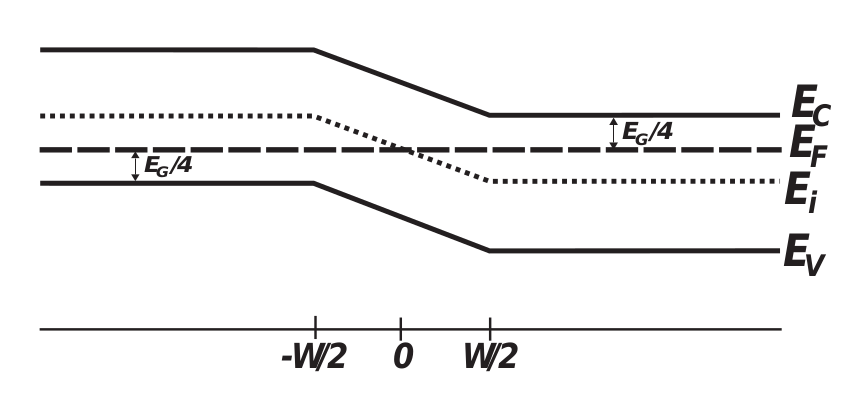
\includegraphics[width=0.7\linewidth]{Cuerpo/Ch_02/02_Ejercicio_15.png}		
\end{center}

\begin{itemize}
	\item[(a)] Si el semiconductor de Si se mantiene a temperatura ambiente, determinar la resistividad del semiconductor para la región \(x > W/2\). Para los electrones en la región \(x > W/2\) que intentan moverse a la región \(x < -W/2\) sin modificar su energía total, ¿cuál es la mínima energía cinética que deben tener?
	\item[(b)] Calcular y representar gráficamente el potencial electrostático y el campo eléctrico en función de \(x\). Explicar si el semiconductor está en equilibrio termodinámico.
	\item[(c)] Responder las siguientes preguntas:
		  \begin{itemize}
			  \item ¿Cuál es la densidad de corriente de electrones (\(J_n\)) y de huecos (\(J_p\)) en \(x = 0\)?
			  \item ¿Existe corriente de arrastre de electrones en \(x = 0\)? Si así fuera, ¿cuál es la dirección del flujo de corriente de arrastre?
			  \item ¿Existe corriente de difusión de electrones en \(x = 0\)? En tal caso, ¿cuál es la dirección del flujo de corriente de difusión?
			\end{itemize}
  \end{itemize}

\rule{\textwidth}{0.1pt} \\[2pt]

\begin{enumerate}[label=\alph*)]
	\item La resisitividad, como hemos visto a lo largo de todos los ejericcios, viene dada por:
	\begin{equation}
		\rho = \frac{1}{q(\mu_n n + \mu_p p)}
	\end{equation}
	Por lo que solo tenemos que calcular $n$ y $p$ para $\mu_n$ y $\mu_p$ dados (valores que tendremos que coger de otro ejercicio). Así pues, obtenemos $n$ y $p$ a partir de las ecuaciones:

	\begin{equation}
		n = n_i e^{(E_F-E_i)/kT} \qquad p = n_i e^{(E_i-E_F)/kT}
	\end{equation}
	Donde conocemos $N_C$ y $N_V$ a 300K (temperatura ambiente) y la diferencia de $E_c-E_F=E_g/4$ y $E_F-E_v=3E_g/4$ en $x>W/2$ (véase diagrama de bandas). Así pues conocemos los valores:

	\begin{equation}
		n= 7.91\times 10^{14} \ \cm^{-3} \tquad p = 4.5\times 10^{14} \ \cm^{-3}
	\end{equation}
	Usando las siguientes movilidades (calculadas con las ecuacioens de portadores mayoritarios/minoritarios previas):
	
	\begin{equation}
		\mu_n = 1290 \ \cm^2 /  \text{V s} \tquad \mu_p = 499 \ \cm^2 /  \text{V s}
	\end{equation}
	tal que la resistividad en $W/2<x$:

	\begin{equation}
		\rho = 5.02 \ \Omega \cm
	\end{equation}
	\textcolor{red}{Da 7.73. En gneral hacen aproximaciones ignorando uno de los portadores.} Ahora solo queda calcualar la energía cinética mínima $T_{\min}$ que deben tener. Como podemos ver la energía de la banda de conducción aumenta de la región $x>W/2$ a la región $x<W/2$. Así pues:

	\begin{equation}
		T_{\min} = E_c(-W/2) - E_c(W/2) = E_g/2 = 0.506 \	 \eV
	\end{equation}
	\item Como sabemos el campo eléctrico viene dado por:
	\begin{equation} 
		\Ecal = \frac{1}{q} \derivadas{E_i}{x}
	\end{equation}
	y el potencial $V(x)=-E_i(x)+V_0$ donde $V_0$ es una constate arbitraria que nos ayuda a redefinir el cero del potencial. Como para calcular la derivada (y $V_0$ siempre nos permite redefinir el cero de $V$) solo necesitamos conocer la \textit{dependencia de $E_i$ con la posición}, podemos escribir 

	\begin{equation}
		E_i = E_{i0} - \frac{E_g}{2} \frac{x}{W}
	\end{equation}
	siendo $E_{i0}$ una constante irrelevante que contiene información de la energía respecto al cero $E_F=0$ eV. Así pues:

	\begin{equation}
		\Ecal = - \frac{1}{q} \frac{E_g}{2W}
	\end{equation}
	Así pues:

	\begin{equation}
		V=V_0 + \frac{E_g}{q} \frac{x}{2W} 
	\end{equation}
	Para ver si está en equilibrio termodinámico tenemos que ver si $J_n=J_p=0$. Veamos que $J_n=0$ implica que:

	\begin{equation}
		J_n = J_n |_{\text{difusion}} +J_n |_{\text{arrastre}} = q\mu_n n \Encal + qD_n\derivadas{n}{x} = 0
	\end{equation}
	De tal modo que, si estamos en equilibrio se tiene que verificar que
	\begin{equation}
		\Ecal_n = \frac{D_n}{\mu_n} \frac{1}{n} \derivadas{n}{x} = 
		\frac{kT}{q} \frac{1}{n} \derivadas{n}{x}
	\end{equation} 
	donde hemos aplicado las reglas de Einstein (válido para el equlibrio y fuera del equlibrio). Ahora solo tenemos que evaluar $n(x)$ y su derivada. Es sencillo de ver que la única dependencia mostrada en el diagrama de bandas:

	\begin{equation}
		n = \left\lbrace
		\begin{array}{ll}
			N_c e^{-\frac{1}{kT}\frac{3E_g}{4}}	& \text{si} \ x<-W/2 \\
			N_c e^{-\frac{1}{kT}\frac{E_g}{4} \parentesis{\frac{-x+W}{W/2}}}	& \text{si} \ -W/2<x<W/2 \\
			N_c e^{-\frac{1}{kT}\frac{E_g}{4}} & \text{si} \ W/2<x
		\end{array} \right.
	\end{equation}
	De lo cual deducimos que la derivada es:

	\begin{equation}
		\derivadas{n}{x} = \left\lbrace
		\begin{array}{ll}
			0	& \text{si} \ x<-W/2 \\
			\frac{1}{kT}\frac{E_g}{4}\frac{2}{W}N_c e^{-\frac{1}{kT}\frac{E_g}{4} \parentesis{\frac{-x+W}{W/2}}}	& \text{si} \ -W/2<x<W/2 \\
			0 & \text{si} \ W/2<x
		\end{array} \right.
	\end{equation}
	Consecuentemente el campo eléctrico:

	\begin{equation}
		\Ecal_n = - \frac{1}{q} \frac{E_g}{2W}   \qquad \text{si} \ - W/2<x<W/2
	\end{equation}  
	Que como podemos ver es la misma expresión. Para los portadores huecos se puede llegar a lo mismo siguiendo los mismos pasos (la única diferencia es que aparecen dos signos menos que se cancelan). Veamos como quedan las gráficas:

	\begin{center}
		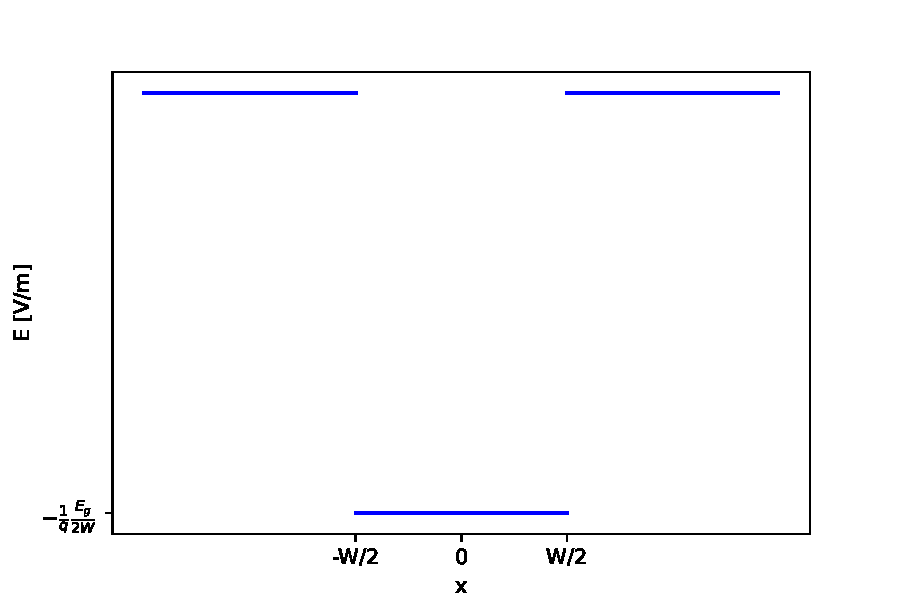
\includegraphics[width=0.7\linewidth]{Cuerpo/Ch_02/02_Ejercicio_15_E(x).pdf}
	\end{center}
	\begin{center}
		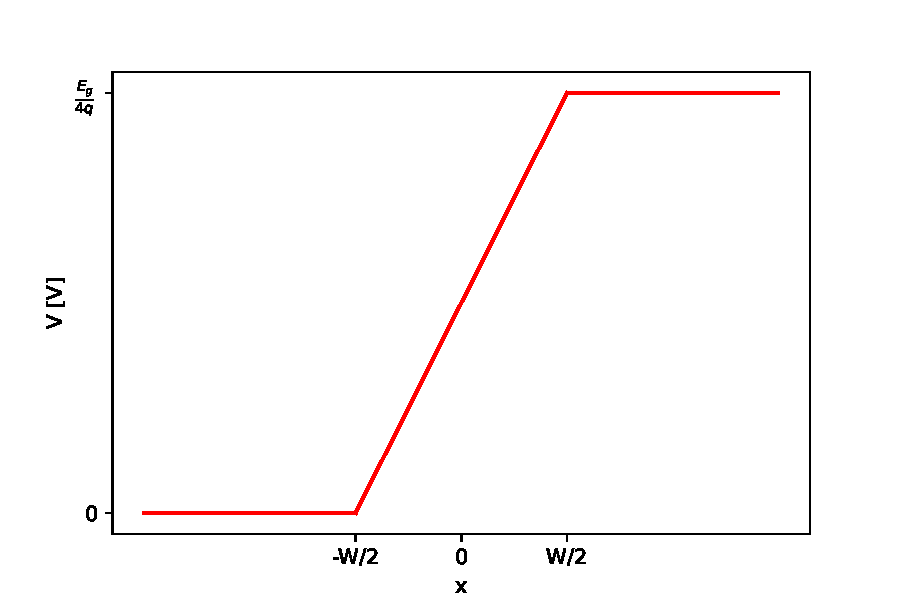
\includegraphics[width=0.7\linewidth]{Cuerpo/Ch_02/02_Ejercicio_15_V(x).pdf}
	\end{center}

	\item Respondemos a cada una de las preguntas:
	\begin{itemize}
		\item La densidad de corriente de electrones y de huecos en $x=0$ es cero, como hemos visto en el apartado anterior. De otra manera no estaríamos en el equilibrio termodinámico.
		\item Corriente de arrastre hay, ya que el campo eléctrico no es nulo (en $x=0$). Así pues: 
		\begin{equation}
			\Jn_n |_{\text{arrastre}} = q \mu_n n \Encal =  - \mu_n \frac{E_g}{2W} N_c  e^{-\frac{1}{kT}\frac{E_g}{2}}  \hnx 
		\end{equation}
		Lógicamente la corriente de arrastre tiene que tener la misma dirección que la corriente eléctrica, ya que aún que la velocidad del electrón tendrá la dirección contraria al campo eléctrico y la corriente de carga tendrá la dirección contraria a la velocidad del electrón. 
		\item Corriente de difusión hay, y en virtud de que $\Jn_n|_{\text{arrastre}}=- \Jn_n|_{\text{difusion}}$, tenemos que
		\begin{equation}
			\Jn_n |_{\text{arrastre}} = - q \mu_n n \Encal =  \mu_n \frac{E_g}{2W} N_c  e^{-\frac{1}{kT}\frac{E_g}{2}}  \hnx 
		\end{equation}
	\end{itemize}
\end{enumerate}


\rule{\textwidth}{0.1pt} \\[2pt]

\subsection{Ejercicio 8}

Interpretación de un diagrama de bandas de energía para un semiconductor de silicio tomando $L=1$ micra:
\begin{center}
	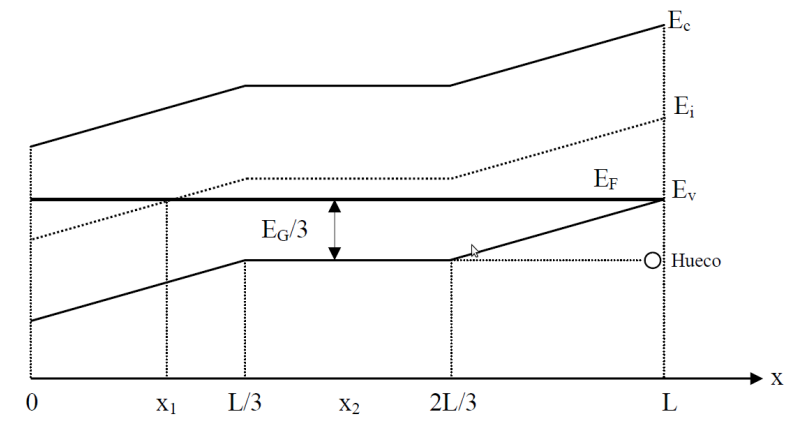
\includegraphics[width=0.7\linewidth]{Cuerpo/Ch_02/02_Ejercicio_16.png}		
\end{center}
\begin{itemize}
	\item[(a)] Calcula y representa graficamente el potencial electrostático y el campo eléctrico en el interior del semiconductor. Determina si el sistema esta o no en equilibrio termodinámico.
	\item[(b)] Calcula si el semiconductor es degenrado en alguna zona. En $x=x_2$, ¿a qué es igual $p$?
	\item[(c)] Captura la densidad de corriente de electrones $J_n$ y la densidad de corriente de arrastre de huecos $J_p^a$ que fluye en $x=x_1$. Determina cuanto vale la energía cinética del hueco que aparece en el diagrama en la posición $x=L$. 
\end{itemize}

\rule{\textwidth}{0.1pt} \\[2pt]


\begin{enumerate}[label=\alph*)]
	\item Queremos calcular el potencial electrostático y el campo eléctrico en el interior del semiconductor. Usamos la misma relación que en el ejercicio anterior:
	\begin{equation}
		\Ecal = \frac{1}{q} \derivadas{E_i}{x}
	\end{equation}
	Veamos que la energía varía como:
	\begin{equation}
		E_i(x) = \left\lbrace \begin{array}{ll}
			\frac{E_{i0}}{L/3-x_1} (x-x_1) \quad & \ \text{si} \ x<L/3 \\
			E_{i0} \quad & \ \text{si} \ L/3<x2L/3 \\
			E_{i0+\frac{E_{i0}}{L/3-x_1} (x-2L/3)} \quad & \ \text{si} \ 2L/3<x
		\end{array} \right.
	\end{equation}
	Recordamos que en $L/3$ tenemos que $E_v=-E_g/3$, y por tanto $E_c=2E_g/3$, tal que $E_{i0}=E_g/6+(3kT/4)\cdot \log(m_n^*/m_p^*)=0.179 \ \eV$, donde hemos redefinido $E_F=0$. Por lo que igual que antes tenemos que el campo eléctrico viene dado por regiones:
	\begin{equation}
		\Ecal(x) = \left\lbrace \begin{array}{ll}
			\frac{E_{i0}}{L/3-x_1} \quad & \ \text{si} \ x<L/3\\
			0 \quad & \ \text{si} \ L/3<x2L/3 \\
			\frac{E_{i0}}{L/3-x_1} \quad & \ \text{si} \ 2L/3<x
		\end{array} \right.
	\end{equation}
	y por tanto:

	\begin{equation}
		V(x) = \left\lbrace \begin{array}{ll}
			V_0 -\frac{E_{i0}}{L/3-x_1} (x-L/3) \quad & \ \text{si} \ x<L/3 \\
			V_0 \quad & \ \text{si} \ L/3<x2L/3 \\
			V_0 -\frac{E_{i0}}{L/3-x_1} (x-2L/3) \quad & \ \text{si} \ 2L/3<x
		\end{array} \right.
	\end{equation}
	Ahora solo tendríamos que hacer el esquema:

	\begin{center}
		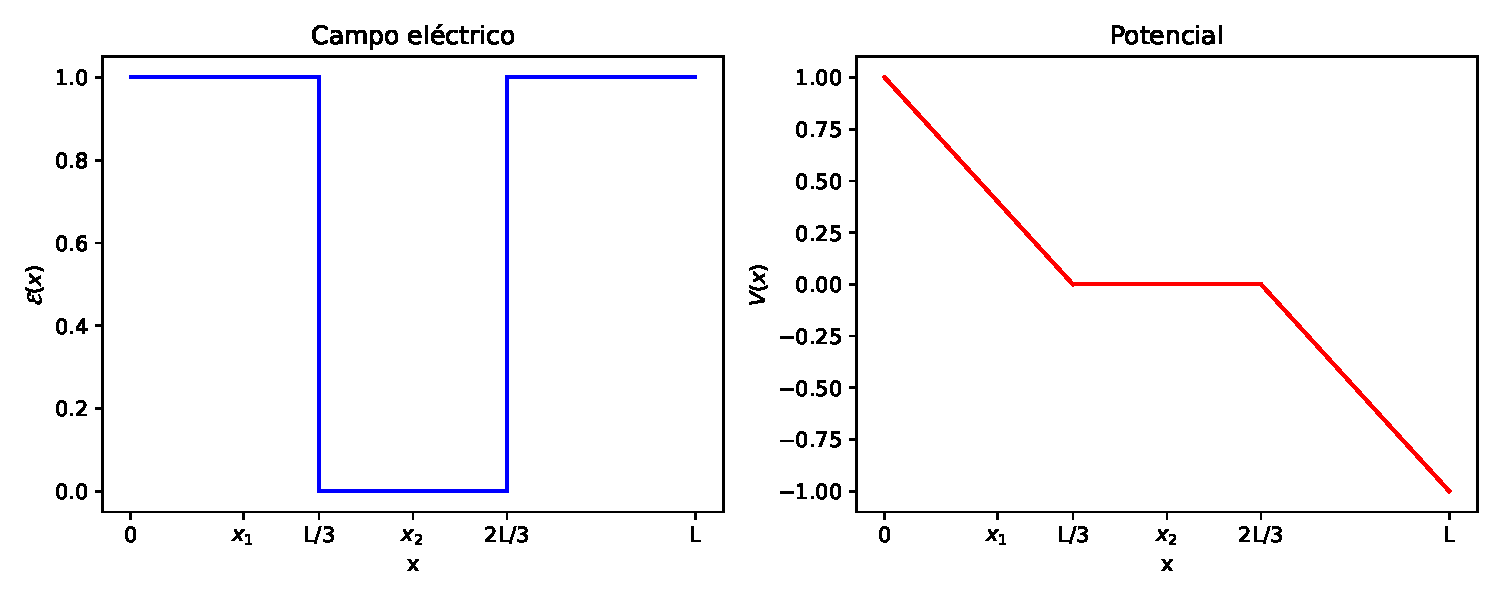
\includegraphics[width=\linewidth]{Cuerpo/Ch_02/02_Ejercicio_16.pdf}
	\end{center}
		
	Para determinar que está en equilibrio basta ver que $\Jn_T=0$ y que $T=\cte$, lo cual es cierto. Para ver que $\Jn=0$ debemos seguir el mismo procedimiento que antes.
	\item  Evidentemente es degenerado en $x=L$, ya que $E_F=E_v$. En $x_2$ tenemos que: 
	\begin{equation}
		p = N_V e^{\frac{E_F-E_v}{kT}} = N_V e^{\frac{E_g}{3kT}} = n_i e^{\frac{E_F-E_i}{kT}}
	\end{equation}
	tal que en $x_2$ tenemos que $E_i=E_{i0}=0.179 \ \eV$. Los datos:

	\begin{equation}
		p = 1.22 \times 10^{13} \ \cm^{-3}
	\end{equation}
	\item Nos piden la densidad de corriente de electrones $J_n$ y la densidad de corriente de huecos en $x=x_1$. Es exactamente igual que en el anterior ejercicio:
	\begin{equation}
		\Jn|_{\text{{arrastre}}} = q \mu_n n \Encal = 0
	\end{equation}
	ya que en $x_1$ no hay corriente. La energía cinética del hueco $T$ viene dada por la diferencia entre $E_v=0$ (en $x=L$) y $-E_g/3$. Así pues:

	\begin{equation}
		T = - \frac{-E_g}{3}
	\end{equation}
	por suponer, ya que no tenemos ningún tipo de motivación para suponer que es así. 

\end{enumerate}

\rule{\textwidth}{0.1pt} \\[2pt]







